\documentclass[12pt]{report}
\RequirePackage[l2tabu, orthodox]{nag}
\usepackage[utf8]{inputenc}
\usepackage[russian]{babel}
\usepackage[top=2cm, bottom=1.5cm, left=2.5cm, right=2.5cm]{geometry}
\usepackage{amssymb,amsthm,framed,mathtools,microtype,titlesec,titletoc,hyperref,tikz,graphicx}
\usepackage[toc]{multitoc}
\numberwithin{equation}{section}
\newtheorem{theorem}{Теорема}[section]
\newtheorem{lemma}{Лемма}[section]
\newtheorem{remark}{Следствие}[section]

\hypersetup{
    colorlinks=true,
    linkcolor=black,
    filecolor=magenta,      
    urlcolor=black,
    pdftitle={Sharelatex Example},
    bookmarks=true,
}

\titleformat{\section}
  {\Large\bfseries} % format
  {}                % label
  {0pt}             % sep
  {\Large}           % before-code


\newcommand{\pvec}[1]{\vec{#1}\mkern2mu\vphantom{#1}}

\makeatletter
\DeclareFontFamily{U}{tipa}{}
\DeclareFontShape{U}{tipa}{m}{n}{<->tipa10}{}
\newcommand{\arc@char}{{\usefont{U}{tipa}{m}{n}\symbol{62}}}%

\newcommand{\arc}[1]{\mathpalette\arc@arc{#1}}

\newcommand{\arc@arc}[2]{%
  \sbox0{$\m@th#1#2$}%
  \vbox{
    \hbox{\resizebox{\wd0}{\height}{\arc@char}}
    \nointerlineskip
    \box0
  }%
}
\makeatother

\makeatletter
\renewcommand{\thesection}{%
  \ifnum\c@chapter<1 \@arabic\c@section
  \else \thechapter.\@arabic\c@section
  \fi
}
\makeatother

\title{Экзамен по математическому анализу.\\Второй семестр}
\date{}

\begin{document}

\maketitle
\tableofcontents

\thispagestyle{empty}


\newpage \section{Вопрос №1}  %%%%%%%%%%%%%%%%% Вопрос 1
\begin{framed}
Теорема о разложении правильной рациональной дроби на простейшие и ее доказательство.\\
\end{framed}
\begin{theorem}[Основная теорема алгебры] Любой многочлен $Q_n(x)$ степени $n$ с действительными коэффициентами представляется в виде
\begin{equation}  \label{eq:1}
Q_n(x) = a_0(x-c_1)^{k_1} \cdot \ldots \cdot (x-c_r)^{k_r}(x^2 + p_1x + q_1)^{s_1} \cdot \ldots \cdot (x^2 + p_tx + q_t)^{s_t},
\end{equation}

где $c_i , \ldots , c_r$ — действительные корни многочлена $Q_n(x)$, квадратные трехчлены $x^2 + p_i x + q_i$ не имеют действительных корней, $k_1 + \dots + k_r + 2(s_1 + \dots + s_t) = n$. 
\end{theorem}


\begin{theorem}
Всякая правильная рациональная дробь представляется в виде
\[ \frac{P_m(x)}{Q_n(x)} = \frac{A_{1,1}}{(x-c_1)^{k_1}} + \dots + \frac{A_{1,k_1}}{x-c_1} + \dots + \left[ \text{аналогично для }c_2, \ldots, c_r\right] + \]
\[ + \frac{M_{1,1}x + N_{1,1}}{(x^2 + p_1x + q_1)^{s_1}} + \dots + \frac{M_{1,s_1}x + N_{1,s_1}}{x^2 + p_1x + q_1} + \dots + \left[ \frac{\text{аналогично для}}{(p_2,q_2), \ldots, (p_t,q_t)}\right]. \]\\

Где в знаменателях стоят сомножетели разложения $\eqref{eq:1}, A_{i,j} , M_{i,j} , N_{i,j}$ — некоторые
числа, зависящие от $P_m(x)$ и $Q_n(x)$.
\end{theorem}

Прежде чем доказать теорему о разложении правильной рациональной дроби сформулируем и докажем две леммы.
\begin{lemma} \label{lemm:1:1}
Если число $a \in \mathbb{R}$  является действительным корнем кратности $k$ многочлена $Q_n(x) = (x-a)^k Q_{n-k}(x)$, то несократимую правильную рациоальную дробь $\dfrac{P_m(x)}{Q_n(x)}$ можно представить в виде

\[\frac{P_m(x)}{Q_n(x)} = \frac{A}{(x-a)^k} + \frac{P_l(x)}{(x-a)^{k-1}Q_{n-k}(x)}, \]

где $A \neq 0$ и $P_l(x)$ ---  многочлен cтепени $l < n - 1$,  т.e. последнее слагаемое является правильной рациональной дробью.
\end{lemma}
\begin{proof}
Добавим к дроби слагаемые $\dfrac{A}{(x-a)^k}~(A \in \mathbb{R})$ с разными знаками и преобразуем выражение:
\[ \frac{P_m(x)}{Q_n(x)} =\frac{P_m(x)}{(x-a)^k Q_{n-k}(x)} + \frac{A}{(x-a)^k} - \frac{A}{(x-a)^k} =  \frac{A}{(x-a)^k} + \frac{P_m(x) - AQ_{n-k}(x)}{(x-a)^k Q_{n-k}(x)}.\]

Второе слагаемое является правильной рациональной дробью, т.к $m < n$ и $n -k < n$. Так как $a$ — корень кратности $k$, то $Q_{n-k}(a) \neq 0$. Так как $\dfrac{P_m(x)}{Q_n(x)}$ --- несократимая дробь, то $P_m(a) \neq 0$. Положим $A = \dfrac{P_m(a)}{Q_{n-k}(a)} \neq 0$. Тогда $P_m(a) - AQ_{n-k}(a) = 0$, а значит, по теореме Безу многочлен $P_m(x) - A Q_{n-k}(x)$ делится на $x-a$. Сократим второе слагаемое на $x-a$:
\begin{equation}\label{eq:2}
\frac{P_m(x) - AQ_{n-k}(x)}{(x-a)^kQ_{n-k}(x)} = \frac{P_l(x)}{(x-a)^{k-1} Q_{n-k}(x)}. 
\end{equation}

Так как эта дробь получена сокращением правильной рациональной дроби, она является правильной (но, возможно, сократимой). 
\end{proof}

\begin{lemma} \label{lemm:1:2}
Если комплексное число $z = \alpha + \beta i~(\beta \neq 0)$ является корнем кратности $s \in \mathbb{N}~(2 \leqslant 2s \leqslant n) $ многочлена $Q_n(x)$ с действительными коэффициентами, то несократимую правильную рациональную дробь $\dfrac{P_m(x)}{Q_n(x)}$ можно представить в виде
\begin{equation}
\frac{P_m(x)}{Q_n(x)} = \frac{Mx + N}{(x^2 + px + q)^s} + \frac{P_l(x)}{(x^2 + px + q)^{s-1} Q_{n-2s}(x)}, \label{eq:3}
\end{equation}

где $x^2 + px + q = (x-z)(x-\bar{z}), Q_{n-2s}(x)$ --- такой многочлен степени $n- 2s$, что
\[ Q_n(x) = (x^2 + px + q)^s Q_{n-2s}(x),~~~~~Q_{n-2s}(z) \neq 0, \]

числа $M, N$ одновременно не обращаются в нуль, а последнее слагаемое в $\eqref{eq:3}$ является правильной рациональной дробью: $l < n - 2$.
\end{lemma}
\begin{proof}
Добавим к дроби слагаемые $\dfrac{(Mx + N)}{(x^2 + px + q)^s}~(M,N \in \mathbb{R})$ с разными знаками и преобразуем выражение:
\begin{equation}\label{eq:4}
\frac{P_m(x)}{Q_n(x)} =\frac{Mx + N}{(x^2 + px + q)^s} + \frac{P_m(x) - (Mx+n)Q_{n-2s}(x)}{(x^2 + px + q)^s Q_{n-2s}(x)}. 
\end{equation}

В знаменателе второго слагаемого в правой части равенства $\eqref{eq:4}$ стоит многочлен степени $n$, а степень многочлена в числителе этого слагаемого меньше $n$, поскольку и $m < n$, и $n - 2s + 1 < n$. Следовательно, это слагаемое является правильной рациональной дробью.\\

Выберем действительные числа $M$ и $N$ так, чтобы многочлен $P_m(x) - (Mx + N) Q_{n-2s}(x)$ делился на $x^2 + px + q$. Это эквивалентно тому, что
\begin{equation}\label{eq:5}
P_m(z) - (Mz + N) Q_{n-2s}(z) = 0, ~~~~~ z = \alpha + \beta i. 
\end{equation}

Тогда и сопряженное $z$ комплексное число $\bar{z} = \alpha - \beta i$ также будет корнем этого уравнения. Поэтому многочлен $P_m(x) - (Mx + N) Q_{n-2s}(x)$ делится на $x^2 + px + q = (x-z)(x-\bar{z})$. Из $\eqref{eq:5}$ следует, что 
\[ M(\alpha + \beta i) + N = \frac{P_m(z)}{Q_{n-2s}(z)} = K + Li,   \]

где $K$ и $L$ --- некоторые действительные числа. Приравнивая в этом равенстве действительные и мнимые части, получаем $M \alpha + N = K$ и $M \beta = L$. Отсюда $M = \dfrac{L}{\beta} $ и $N = K - \dfrac{\alpha L}{\beta}$. Числа $M$ и $N$ одновременно не обращаются в нуль, так как в противном случае $P_m(z) = 0$ и дробь $\dfrac{P_m(x)}{Q_n(x)}$ сократима, а это противоречит условию леммы. При таком выборе $M$ и $N$ второе слагаемое в правой части $\eqref{eq:4}$ можно сократить на $x^2 + px + q$, записав его в виде
\begin{equation}\label{eq:6}
\frac{P_m(x) - (Mx + N) Q_{n-2s} (x)}{(x^2 + px + q)^s Q_{n-2s}(x)} = \frac{P_l(x)}{(x^2 + px + q)^{s-1} Q_{n-2s}(x)}, 
\end{equation}

где $P_l(x) = \dfrac{P_m(x) - (Mx + N) Q_{n-2s}(x)}{x^2 + px + q}$. Рациональная дробь в правой части $\eqref{eq:6}$ получена сокращением правильной рациональной дроби с действительными коэффициентами на множитель $x^2 + px + q$, где $p$ и $q$ --- действительные числа, и поэтому является правильной рациональной дробью с действительными коэффициентами.
\end{proof}

\begin{proof}[Доказательство теоремы]
К правильной рациональной дроби в правой части $\eqref{eq:2}$ при $k > 1$ можно вновь применить лемму \ref{lemm:1:1} и в итоге получить
\begin{equation}\label{eq:7}
\frac{P_m(x)}{Q_n(x)} = \frac{A}{(x-a)^k} + \frac{A_1}{(x-a)^{k-1}} + \ldots + \frac{A_{k-1}}{x-a} + \frac{P_{l_1}(x)}{Q_{n-k}(x)}.
\end{equation}

Здесь $\dfrac{P_{l_1}(x)}{Q_{n-k}(x)}$ --- несократимая правильная рациональная дробь, так как в ином случае правая часть в $\eqref{eq:7}$ после ее приведения к общему знаменателю является сократимой дробью, а это противоречит условию леммы. Если многочлен $Q_{n-k}(x)$ имеет другие действительные корни, то к последней дроби в правой части $\eqref{eq:7}$ также применима лемма \ref{lemm:1:1}. И т.д.\\

Если многочлен $Q_n(x)$  не имеет действительных корней, а имеет комплексные корни, то применима лемма \ref{lemm:1:2}. Ко второму слагаемому в правой части $\eqref{eq:3}$ при $s > 1$ можно вновь применить лемму \ref{lemm:1:2} и получить
\[ \frac{P_m(x)}{Q_n(x)} = \frac{Mx + N}{(x^2 + px + q)^s} + \frac{M_1x + N_1}{(x^2 + px + q)^{s-1}} + \ldots + \frac{M_{s-1}x + N_{s-1}}{x^2 + px + q} + \frac{P_s(x)}{Q_{n-2s}(x)},\]

где $\dfrac{P_s(x)}{Q_{n-2s} (x)}$ ---  несократимая правильная рациональная дробь. Многочлен $Q_{n-2s}(x)$ имеет другие комплексные корни, а значит, к этой дроби также применима лемма \ref{lemm:1:2}. И т.д.
\end{proof}

\newpage \section{Вопрос №2} %%%%%%%%%%%%%%%%% Вопрос 2
\begin{framed}Интегрирование простейших дробей и рациональных функций.
\end{framed}
\textbf{Рациональными} называют функции вида
\[f(x) = \frac{P_m(x)}{Q_n(x)},~~~~
\begin{aligned}
P_m(x) &= b_0x^m + b_1 x^{m-1} + \ldots + b_{m-1}x +b_m,\\
Q_n(x) &= a_0 x^n + a_1 x^{n-1} + \ldots + a_{n-1}x + a_n.
 \end{aligned}\]

\textbf{Простейшие рациональные дроби:}
\[ 1)~\frac{A}{x-a},~~~2)~\frac{B}{(x-a)^k},~~~3)~\frac{Mx + N}{x^2 + px + q}~~~4)~\frac{Mx+N}{(x^2 + px + q)^k},~~~k>1\]

Схема интегрирования рациональных функций: сначала функцию представляют в виде суммы простейших дробей, а затем интегрируют каждое слагаемое полученного разложения.

Если $n > m \geqslant 0$,  рациональную дробь называют \textbf{правильной}, в противном случае --- \textbf{неправильной}. Используя правило деления многочленов, неправильноую рациональную дробь можно предстваить в виде суммы многочлена $P_{m-n}$ степени  $m-n$ и некоторой правильной дроби, т.е.
\[ \frac{P_m(x)}{Q_n(x)} = P_{m-n}(x) + \frac{P_l(x)}{Q_n(x)},\]

где многочлен $P_l(x)$ имеет степень $l < n$.

\begin{theorem}[Теорема Безу]
Если $a$ --- корень многочлена $P(x)$, то многочлен $P(x)$ делится на $x-a$ без остатка.
\end{theorem}
 
Натуральное число $k$ называют \textbf{кратностью} корня $a$ многочлена $P(x)$, если существует такой многочлен $Q(x)$, что
\[ P(x) = (x-a)^k Q(x),~~~~Q(a) \neq 0.\]

Теорема Безу верна и в случае действительного, и в случае комплексного корня. Пусть многочлен $Q_n(x)$ степени $n$ с действительными коэффициентами имеет комплексный корень $z = \alpha + \beta i~(\alpha, \beta \in \mathbb{R},~\beta \neq 0$, $i$ --- \textbf{мнимая единица}, $i^2 = -1$) кратности $k \in \mathbb{N}$. Но тогда сопряженное с этим корнем комплексное число $\bar{z} = \alpha - \beta i$ является для данного многочлена корнем той же кратности, т.е. многочлен $Q_n(x)$ делится на многочлен
\[ ((x-z)(x-\bar{z}))^k = (x^2 + px + q)^k,\]

где $p = -2a$ и $q = \alpha^2 + \beta^2$ --- действительные числа.\\

\textbf{Алгоритм интегрирования рациональных функций:}

\begin{enumerate}
\item [0.] В случае, если необходимо проинтегрировать недробное рациональное выражение, перейти к шагу 4
\item Выделить правильную дробь (если необходимо)
\item Найти вид разложения на простейшие дроби
\item Найти коэффициенты разложения
\item Проинтегрировать каждое слагаемое
    \begin{enumerate}
    \item [4.1] Воспользоваться методом интегрирования подведением под знак дифференциала или замены переменных, чтобы получить табличный интеграл
    \item [4.2] ???
    \item [4.3] PROFIT
    \end{enumerate}
\end{enumerate}

\newpage

\newpage \section{Вопрос №3}  %%%%%%%%%%%%%%%%% Вопрос 3
\begin{framed}Дать определение интеграла Римана. Доказать его свойства: линейность и интеграл от константы.
\end{framed}

Пусть функция $f(x)$ определена на отрезке $[a,b]$. Конечное множество точек $a = x_0 < x_1 < \ldots < x_n = b$ называют разбиением отрезка $[a,b]$ и обозначают $P = (x_0, x_1, \ldots, x_n)$. Для каждого $i = 1, \ldots, n$ отрезок $[x_{i-1}, x_i] \subseteq [a,b]$ назовем частичным отрезком разбиения $P$ и обозначим через $\Delta_i$. Его длину обозначим через $\Delta x_i = x_i - x_{i-1}~(i = 1, \ldots, n)$. Число $\lambda = max_{i = 1, \ldots, n}\Delta x_i $ называют параметром разбиения (или диаметром разбиения) $P$. Заметим, что $\lambda \geqslant (b-a)/n$.\\

Пусть на каждом частичном отрезке произвольным образом выбрана точка $\xi_i \in [x_{i-1}, x_i]$. Пару $(P, \xi)$, где $\xi = (\xi_1, \ldots, \xi_n)$, называют разбиением с отмеченными точками.\\

Сумму 
\[ \sigma(f;P, \xi) = \sum\limits_{i=1}^{n}f(\xi_i)\Delta x_i\]

называют интегральной суммой для функции $f(x)$, соответствующей разбиению $P = (x_0, \ldots, x_n)$ с отмеченными точками $\xi = (\xi_1, \ldots, \xi_n)$ отрезка $[a,b]$.\\

В множестве $\mathcal{P}$ разбиений с отмеченными точками данного отрезка $[a,b]$ рассмотрим следующую базу $\{b_d\}, d> 0:$
\[ b_d = \{ (P, \xi) \in \mathcal{P} : \lambda < d\}.\]

Проверим, что $\{b_d\}, d> 0$ --- действительно база в $\mathcal{P}$:
\begin{enumerate}
\item [1)] Для любого $d > 0$ элемент $b_d$ не пуст, так как существует разбиение отрезка $[a,b]$ на $n = [(b-a)/d] +1$ отрезков одинаковой длины $(b-a)/n <d$. В качестве отмеченных точек $\xi_i$ всегда можно взять середины отрезков. Поэтому $b_d \neq \varnothing$.
\item [2)] Если $d_1 >0$, $d_2 > 0$ и $d = min(d_1,d_2)$, то $b_{d/2} \subset b_d = b_{d_1} \cap b_{d_2}$ и $b_{d/2} \neq b_d$.
\end{enumerate}

Будем обозначать эту базу через $\lambda \to 0$. Предел по этой базе значений интегральных сумм для функции $f$, отвечающих разбиению с отмеченными точками отрезка $[a,b]$, называют \textbf{интегралом Римана (определенным интегралом)} от функции $f$ на отрезке $[a,b]$ и обозначают
\[ \int_{a}^b f(x) dx = \lim_{\lambda \to 0}\sum_{i=1}^n f(\xi_i) \Delta x_i.\]

\begin{theorem}[Линейность интеграла Римана] \label{th:3:1}
Пусть функции $f_1$и $f_2$ интегрируемы на отрезке $[a,b]$. Тогда при $\alpha_1, \alpha_2 \in \mathbb{R}$ функция $\alpha_1 f_1 + \alpha_2 f_2 $ также интегрируема на отрезке $[a,b]$ и 
\begin{equation}\label{eq:3:1}
\int_a^b (\alpha_1 f_1 + \alpha_2 f_2) (x) ~dx = \alpha_1 \int_a^b f_1(x) ~dx + \alpha_2 \int_a^b f_2(x)~dx. 
\end{equation}
\end{theorem}
\begin{proof} Пусть $a < b$. Для некоторого разбиения $P = (x_0, \ldots, x_n)$ с отмеченными точками $\xi = (\xi_1, \ldots, \xi_n)$ отрезка $[a,b]$ имеем равенство
\begin{equation}\label{eq:3:2}
\sum_{i=1}^n(\alpha_1f_1(\xi_i) + \alpha_2 f_2 (\xi_i))\Delta x_i = \alpha_1 \sum_{i=1}^n f_1 (\xi_i) \Delta x_i + \alpha_2 \sum_{i=1}^n f_2 (\xi_i) \Delta x_i.
\end{equation}

В силу интегрируемости функций $f_1(x)$ и $f_2(x)$ на отрезке $[a,b]$, стоящие в правой части этого равенства интегральные суммы имеют пределы по базе $\lambda \to 0$. Но тогда существует конечный предел по этой базе и для интегральной суммы в левой части этого равенства, что в силу определения доказывает интегрируемость функции $\alpha_1f_1(x) + \alpha_2 f_2(x)$ на отрезке $[a,b]$. Переходя в обеих частях равенства \eqref{eq:3:2} к пределу, получаем равенсто из утверждения теоремы.\\

При $a = b$ все три интеграла в \eqref{eq:3:1} равны нулю. А при $a > b$, меняя местами $a$ и $b$, меняем знаки всех трех интегралов, а значит, этот случай сводится к случаю $a < b$.
\end{proof}

\begin{theorem}[Интеграл от константы]
\[ \int_a^b c~dx = c(b-a).\]
\end{theorem}
\begin{proof}
Интегральная сумма для константы не зависит от выбора разбиения $P$ и отмеченных точек $\xi$ и равна
\[ \sigma(f;P;\xi) = \sum_{i=1}^n c\Delta x_i = c(b-a).\]

Из теоремы о пределе постоянной функции получаем указанную формулу.
\end{proof}
\newpage \section{Вопрос №4} %%%%%%%%%%%%%%%%% Вопрос 4
\begin{framed}
Необходимое условие интегрируемости и его доказательство
\end{framed}
\begin{theorem}[необходимое условие интегрируемости]
\[ f \subset \mathcal{R}[a,b] \implies f \text{ ограничена на отрезке } [a,b].\]
\end{theorem}

\begin{proof}
Предположим противное: функция $f(x)$ интегрируема на отрезке $[a,b]$ и не ограничена на этом отрезке. Согласно определению интегрируемости, существует конечный предел интегральных сумм для этой функции на данном отрезке. Из теоремы о локальной ограниченности функции, имеющей предел, существует элемент базы $b_d$, на котором интегральная сумма ограничена, т.е.
\begin{equation}\label{eq:4:1}
\exists c > 0 ~~~ \left( \lambda(P) < d \implies |\sigma(f;P;\xi)| < c\right).
\end{equation}

Выберем одно из таких разбиений $(P, \xi)$  с отмеченными точками. Поскольку функция $f(x)$ не ограничена на отрезке $[a, b]$,
 то найдется частичный отрезок $\Delta_j$, на котором функция $f(x)$ является неограниченной. Разобьем интегральную сумму на два слагаемых и используем неравенство треугольника:
\begin{equation}
\begin{aligned} \label{eq:4:2}
|\sigma(f;P;\xi)| &=  \left| f(\xi_j) \Delta x_j + \sum_{i\neq j} f(\xi_i) \Delta x_i \right| \geqslant\\
&\geqslantя |f (\xi_j) \Delta x_j| - \left|  \sum_{i\neq j} f(\xi_i) \Delta x_i \right| = |f(\xi_j)| \Delta x_j - c_1,
\end{aligned} 
\end{equation}

где $c_1$ --- значение второго слагаемого. Меняя только точку $\xi_j \in \Delta_j$, но не меняя остальные элементы разбиения $(P, \xi)$, слагаемое $f(\xi_j) \Delta x_j$ в интегральной сумме можно сделать сколь угодно большим по абсолютной величине, но это противоречит неравенствам \eqref{eq:4:1} и \eqref{eq:4:2}. Возникшее противоречие опровергает принятое предположение и доказывает утверждение теоремы.
\end{proof}

\newpage \section{Вопрос №5} %%%%%%%%%%%%%%%%% Вопрос 5
\begin{framed}
Критерий интегрируемости, его доказательство.
\end{framed}

\textbf{Колебанием функции $f$ на множестве $E$} называют число
\[ \omega(f;E) = \sup_{x', x'' \in E} | f(x') - f(x'') |.\]

\begin{theorem}[Критерий интегрируемости]
В введенных обозначениях
\[ f \in \mathcal{R}[a,b] \iff \lim_{\lambda \to 0} \sum_{i=1}^n \omega(f; \Delta_i) \Delta x_i = 0. \]
\end{theorem}
Докажем сначала два вспомогательных утверждения. Пусть разбиение $\tilde{P}$ отрезка $[a,b]$ получено из разбиения $P$ только добавлением некоторых новых точек. Будем называть разбиение $\tilde{P}$ \textbf{продолжением} разбиения $P$.\\

\begin{lemma}
Пусть $\tilde{P}$ --- продолжение разбиения $P$. $\xi, \tilde{\xi}$ --- отмеченные точки разбиений $P, \tilde{P}$ соответственно. Тогда
\begin{equation}\label{eq:5:1}
\left|\sigma(f; \tilde{P}, \tilde{\xi}) - \sigma(f; P, \xi)\right| \leqslant \sum_{i=1}^n \omega (f; \Delta_i) \Delta x_i. 
\end{equation}
\end{lemma}
\begin{proof}
Введем следующие обозначения. При построении продолжения $\tilde{P}$ некоторые (может и не все) частичные отрезки $\Delta_i = [x_{i-1}, x_i]$ разбиения $P$ сами подвергаются разбиению $x_{i-1} = x_{i0} < x_{i1} < \ldots < x_{ik_i} = x_i$. Поэтому будем нумеровать точки разбиения $\tilde{P}$  двумя индексами. В записи $x_{ij}$ первый индекс означает, что $x_{ij}  \in \Delta_i$, а второй индекс есть порядковый номер точки на отрезке $\Delta_i$. Положим также $\Delta x_{ij} = x_{ij} - x_{ij - 1}$ и $\Delta_{ij} = [x_{ij - 1}, x_{ij}]$.\\

Пусть $\xi = (\xi_1, \ldots, \xi_n)$ и $\tilde{\xi} = (\xi_{11}, \ldots, \xi_{nk_n})$  --- отмеченные точки разбиений $P$ и $\tilde{P}$ соответственно. Нумерация точек $\tilde{\xi}$ выбрана так, что $\xi_{ij} \in \Delta_{ij}$. Используя определения, неравенство треугольника и равенства $\Delta x_i = \Delta x_{i1} + \ldots + \Delta x_{ik_i}$ при $i = 1, \ldots, n$, получаем
\[ | \sigma(f; \tilde{P}, \tilde{\xi}) - \sigma(f; P; \xi) | = \left| \sum_{i=1}^n \sum_{j=1}^{k_i} f(\xi_{ij}) \Delta x_{ij} - \sum_{i=1}^n f(\xi_i) \Delta x_{i}  \right| =\]
\[= \left| \sum_{i=1}^n \sum_{j=1}^{k_i}f(\xi_{ij}) \Delta x_{ij} - \sum_{i=1}^n \sum_{j=1}^{k_i} f(\xi_i) \Delta x_{ij} \right| = \left| \sum_{i=1}^n \sum_{j=1}^{k_i} (f(\xi_{ij}) - f(\xi_i)) \Delta x_{ij} \right| \leqslant \]
\[ \leqslant \sum_{i=1}^n \sum_{j=1}^{k_i} \left| f(\xi_{ij}) - f(\xi_i) \right| \Delta x_{ij} \leqslant \sum_{i=1}^n \sum_{j=1}^{k_i} \omega(f; \Delta_i) \Delta x_{ij} = \sum_{i=1}^n \omega (f; \Delta_i) \Delta x_i. \]
\end{proof}

Пусть $f \in \mathcal{R}[a,b]$, а $P$ --- произвольное разбиение отрезка $[a,b]$. Тогда из необходимого условия интегрируемости следует ограниченность функции $f$ на отрезке $[a,b]$, и поэтому определены значения:
\[ M_i = \sup_{x \in \Delta_i} f(x),~~~ m_i = \inf_{x \in \Delta_i} f(x),~~~ S(f;P) = \sum_{i = 1}^n M_i \Delta x_i, ~~~ s(f; P) = \sum_{i = 1}^n m_i \Delta x_i.\]

Суммы $S(f;P)$ и $s(f; P)$ называют \textbf{верхней} и \textbf{нижней суммами Дарбу} для функции $f(x)$, соответствующими фиксированному разбиению $P$. Из определений имеем
\begin{equation} \label{eq:5:2}
s(f;P) \leqslant S(f;P).
\end{equation}

\begin{lemma}
Пусть $f \in \mathcal{R}[a,b]$, а $P$ --- какое-либо разбиение отрезка $[a,b]$. Тогда для любого $\varepsilon > 0$ найдется такой набор $\xi$ отмеченных точек, что
\begin{equation} \label{eq:5:3}
S(f;P) < \sigma (f; P, \xi) + \varepsilon.
\end{equation}
\end{lemma}
\begin{proof}
По определению чисел $M_i$ для каждого $i$ найдется точка $\xi_i \in \Delta _i$, в которой $M_i < f(\xi_i) + \dfrac{\varepsilon}{b - a}$. Тогда для $\xi = (\xi_1, \ldots, \xi_n)$ имеем
\[ S(f;P) = \sum_{i=1}^n M_i \Delta x_i < \sum_{i=1}^n \left( f(\xi_i) + \frac{\varepsilon}{b - a}\right) \Delta x_i = \sum_{i = 1}^n f(\xi_i) \Delta x_i + \varepsilon = \sigma(f; P, \xi) + \varepsilon. \]
\end{proof}

Аналогично доказывается, что для любого $\varepsilon > 0$ найдется такой набор $\xi'$ отмеченных точек, что
\begin{equation}\label{eq:5:4}
\sigma(f;P, \xi') - \varepsilon < s(f;P). 
\end{equation}

\begin{proof}[Доказательство теоремы] Основано на критерии Коши существования предела по базе.\\

$\Leftarrow$: Пусть
\[ \lim_{\lambda \to 0} \sum_{i=1}^n \omega(f; \Delta_i) \Delta x_i = 0.\]

По определению предела по базе для любого $\varepsilon > 0$ найдется число $\delta > 0$ такое, что для любого разбиения $(P, \xi)$ с отмеченными точками отрезка $[a,b]$, параметр которого $\lambda < \delta$, имеет место соотношение
\begin{equation} \label{eq:5:5}
\left| \sum_{i=1}^n \omega(f; \Delta_i) \Delta x_i\right| < \frac{\varepsilon}{2}.
\end{equation}

Если теперь $(P', \xi')$ и $(P'', \xi'')$  --- разбиения с отмеченными точками отрезка $[a,b]$, параметры которых удовлетворяют условиям $\lambda' < \delta,~ \lambda'' < \delta$, то рассмотрим разбиение $\tilde{P} = P' \cup P''$, являющееся продолжением обоих разбиений $P', P''$. Из неравенств \eqref{eq:5:1} и \eqref{eq:5:4} следует, что
\[ \left|\sigma(f; \tilde{P}, \tilde{\xi}) - \sigma(f; P', \xi') \right| < \frac{\varepsilon}{2}, ~~~~ \left|\sigma(f; \tilde{P}, \tilde{\xi}) - \sigma(f; P'', \xi'')\right| < \frac{\varepsilon}{2}. \]

А значит, из неравенства треугольников получаем
\[ \left| \sigma(f; P', \xi') - \sigma(f; P'', \xi'')\right| < \varepsilon.\]

В силу критерия Коши существует предел $\lim\limits_{\lambda \to 0} \sigma(f; P, \xi)$, т.е. $f \in \mathcal{R}[a,b]$.\\

$\Rightarrow$: Если  $f \in \mathcal{R}[a,b]$, то существует предел  $\lim\limits_{\lambda \to 0} \sigma(f; P, \xi)$. В силу критерия Коши для любого $\varepsilon > 0$ найдется такое число $\delta > 0$, что для разбиений $(P, \xi')$ и $(P, \xi'')$ с отмеченными точками отрезка $[a,b]$, параметр которых $\lambda < \delta$, имеет место соотношение
\begin{equation} \label{eq:5:6}
\left| \sigma(f;P, \xi') - \sigma(f;P, \xi'')\right| < \varepsilon.
\end{equation}


Из соотношений \eqref{eq:5:2} - \eqref{eq:5:4} и \eqref{eq:5:6} следует, что
\[ \left| S(f;P) - s(f;P)\right| \leqslant | \sigma(f;P, \xi') - \sigma(f; P, \xi'') + 2 \varepsilon | < 3 \varepsilon,\]

а значит
\[ \lim_{\lambda \to 0} \left( S(f;P) - s(f;P)\right) = 0.\]

Но $\omega(f;\Delta_i) = M_i - m_i$, поэтому
\[ \lim_{\lambda \to 0} \sum_{i = 1}^n \omega(f; \Delta_i) \Delta x_i =  \lim_{\lambda \to 0} \sum_{i = 1}^n (M_i - m_i) \Delta x_i =\lim_{\lambda \to 0} \left( S(f;P) - s(f;P)\right) = 0.\]
\end{proof}

\newpage \section{Вопрос №6} %%%%%%%%%%%%%%%%% Вопрос 6
\begin{framed}
Доказательство интегрируемости непрерывных функций и функций с конечным числом
точек разрыва.
\end{framed}
\begin{remark}Если функция $f(x)$ непрерывна на отрезке $[a,b]$, то она интегрируема на этом отрезке.
\end{remark}
\begin{proof}
По теореме Кантора, поскольку функция $f(x)$ непрерывна на отрезке $[a,b]$, она равномерно непрерывна на нем. Поэтому для любого $\varepsilon > 0$ найдется такое $\delta = \delta(\varepsilon) > 0$, что отрезок $[a,b]$ можно разбить на частичные отрезки длиной меньше $\delta$, на каждом из которых колебание функции $f(x)$ будет меньше $\dfrac{\varepsilon}{b - a}$, т.е. при диаметре $\lambda(P) < \delta$ разбиения $P$ будет выполнено неравенство $0 \leqslant \omega(f; \Delta_i) < \dfrac{\varepsilon}{b-a}$. Умножая это неравенство на длину $\Delta x_i > 0$  частичного отрезка и суммируя по $i$, получаем
\[ 0 \leqslant \sum_{i = 1}^n \omega(f; \Delta_i) \Delta x_i < \sum_{i = 1}^n \frac{\varepsilon}{b-a} \Delta x_i = \varepsilon,\]

что в силу критерия интегрируемости доказывает утверждение теоремы.
\end{proof}

\begin{remark} Ограниченная с конечным числом точек разрыва на отрезке функция интегрируема на этом отрезке.
\end{remark}
\begin{proof}
Пусть функция $f$ ограничена и имеет $k$ точек разрыва на отрезке $[a,b]$. Проверим выполнимость условия критерия интегрируемости.\\

Так как функция $f$ ограничена, то определено и конечно колебание $\omega(f; [a,b])$ этой функции на отрезке $[a,b]$. Обозначим его через $\omega$. При заданном $\varepsilon > 0$ посторим $\delta_1$-окрестности каждой из $k$ точек разрыва функции $f$ на $[a,b]$ (значение $\delta_1$ выберем позже). Дополнительное к объединению этих окрестностей множество точек отрезка $[a,b]$ состоит из конечного числа отрезков, на каждом из которых $f$ непрерывна и, значит, равномерно непрерывна. Поскольку таких отрезков конечное число, по $\varepsilon > 0$ можно указать $\delta_2 = \delta_2(\varepsilon) > 0$ так, что на любом отрезке $\Delta$, длина которого меньше $\delta_2$  и который полностью содержится в одном из указанных выше отрезков непрерывности $f$, будем иметь $\omega(f; \Delta) < \dfrac{\varepsilon}{2(b-a)}$.\\

Возьмем теперь число $\delta = \min\{\delta_1, \delta_2\}$. Пусть $P$ --- произвольное разбиение отрезка $[a,b]$, для которого $\lambda(P) < \delta$. Сумму из критерия интегрируемости, отвечающую разбиению $P$, разобьем на две части:
\[ \sum_{i = 1}^n \omega(f; \Delta_i) \Delta x_i = \sum_{i'} \omega(f; \Delta_i) \Delta x_i + \sum_{i \neq i'} \omega(f; \Delta_i) \Delta x_i.\]

В сумму $\sum\limits_{i'}$ включим те слагаемые, которые отвечают отрезкам $\Delta_i$ разбиения $P$, не имеющим общих точек с постороенными $\delta_1$-окрестностями точек разрыва. Для таких отрезков $\Delta_i$ имеем $\omega(f; \Delta_i) < \dfrac{\varepsilon}{2(b-a)}$, поэтому
\[ \sum_{i'} \omega(f; \Delta_i) \Delta x_i < \frac{\varepsilon}{2(b-a)} \sum_{i'} \Delta x_i < \frac{\varepsilon}{2(b-a)} (b-a) = \frac{\varepsilon}{2}.\]

Сумма длин оставшихся отрезков разбиения $P$ меньше
\[ (\delta + 2 \delta_1 + \delta)k \leqslant 4 \delta_1 k = \frac{\varepsilon}{2\omega},\]

если положить $\delta_1 = \dfrac{\varepsilon}{8\omega k}$. Поэтому
\[ \sum_{i \neq i'} \omega(f; \Delta_i) \Delta x_i \leqslant \omega \sum_{i \neq i'} \Delta x_i < \omega \frac{\varepsilon}{2\omega} = \frac{\varepsilon}{2}.\]

Таким образом, мы получаем, что при $\lambda(P) < \delta$
\[ \sum_{i = 1}^n \omega(f; \Delta_i) \Delta x_i < \varepsilon, \]

т.е. выполнено условие критерия интегрируемости поэтому $f \in \mathcal{R}[a,b]$.
\end{proof}

\newpage \section{Вопрос №7} %%%%%%%%%%%%%%%%%%%%% Вопрос 7

\begin{framed}
Сформулировать и доказать свойство аддитивности определенного интеграла.
\end{framed}

\begin{theorem} \label{th:7:1}
Если функция интегрируема на отрезке $[a,b]$, то она интегрируема и на любом меньшем отрезке $[c,d] \subset [a,b]$.
\end{theorem}
\begin{proof}
Пусть $P$ --- разбиение отрезка $[c,d]$. Добавив к $P$ некоторые точки, достроим $P$ до разбиения $P'$ отрезка $[a,b]$, но так, чтобы диаметр $\lambda'$ разбиения $P'$ был не больше диаметра $\lambda$ разбиения $P$. Тогда
\begin{equation}\label{eq:7:1}
0 \leqslant \sum_{P} \omega(f |_{[c,d]}; \Delta_i) \Delta x_i \leqslant \sum_{P'} \omega(f; \Delta_i) \Delta x_i, 
\end{equation}

где $\sum\limits_{P}$ --- сумма по всем отрезкам разбиения $P$, а $\sum\limits_{P'}$ --- сумма по всем отрезкам разбиения $P'$.\\

Так как $\lambda \geqslant \lambda' \geqslant 0$, то $\lambda' \to 0$ при $\lambda \to 0$. Переходя в неравенстве \eqref{eq:7:1} к пределу по базе $\lambda \to 0$ и используя теорему о пределе промежуточной функции и критерий интегрируемости, получаем $f \in \mathcal{R} [a,b] \implies f \in \mathcal{R} [c,d].$
\end{proof}

Определенный интеграл Римана обобщается на случай $a \geqslant b$, при этом перестановка пределов интегрирования в определенном интеграле изменяет его знак, а интегралу с $a = b$ приписывают нулевое значение:
\begin{equation}\label{eq:7:2}
\int_a^b f(x)~dx = - \int_b^a f(x)~dx \text{ при } a > b, ~~~~~ \int_a^a f(x)~dx = 0.
\end{equation}

\begin{theorem} \label{th:7:2}
Если функция $f(x)$ интегрируема на наибольшем из отрезков $[a,b]$, $[a,c]$, $[c,b]$, то она интегрируема на двух других отрезках и справедливо равенство
\begin{equation}\label{eq:7:3}
\int_a^b f(x)~dx = \int_a^c f(x) ~dx + \int_c^b f(x)~dx, 
\end{equation}

каково бы ни было взаимное расположение точек $a$, $b$ и $c$.
\end{theorem}
\begin{proof}
Предположим сначала, что $a < c < b$ и функция $f(x)$  интегрируема на отрезке $[a,b]$. На основании теоремы \ref{th:7:1} заключаем, что $f(x)$ интегрируема на отрезках $[a,c]$ и $[c,b]$. Поэтому в дальнейших рассуждениях можно использовать некоторый специальный вид разбиений этих отрекзов.

\begin{center}
\begin{tikzpicture}\label{pic:7:1}
\draw[thick, ->] (-3.5, 0) -- (3,0) node[below]{x};
\draw (2.49, 0) -- (2.49, .25) node at (2.49, -.2) {$b$};
\draw (-2.98, 0) -- (-2.98, .25) node at (-2.98, -.2) {$a$};
\draw (-1, 0) -- (-1, .25) node at (-1, -.2) {$c$};
\draw (-1, 0) arc (70:110:2.9cm) node at (1, .6) {$T_m$};
\draw (2.5, 0) arc (-70:-110:8cm) node at (-.2, -1) {$T_n$};
\draw (2.5, 0) arc (70:110:5.1cm) node at (-2, .6) {$T_k$};
\draw node at (0, -2) {Рис. 1};
\end{tikzpicture} 
\end{center}

Рассмотрим разбиение $T_n$ отрезка $[a,b]$ на $n$ частичных отрезков, причем точку $c$ будем считать одной из точек деления этого отрезка (\hyperref[pic:7:1]{рис. 1}). Пусть при этом $T_k$ и $T_m$ --- разбиения отрезков $[a,c]$ и $[c,b]$ на $k$ и $m$ частичных отрезков соответственно $(k + m = n)$. Тогда интегральную сумму функции $f(x)$ для разбиения $T_n = T_k \cup T_m$ отрезка $[a,b]$ можно записать в виде
\begin{equation} \label{eq:7:4}
\sum_{i=1}^n f(\xi_i) \Delta x_i = \sum_{i=1}^k f(\xi'_i) \Delta x'_i + \sum_{i=1}^m f(\xi''_i) \Delta x''_i,
\end{equation}

где первое слагаемое справа соответствует разбиению $T_k$ отрезка $[a,c]$, а второе --- разбиению $T_m$ отрезка $[c,b]$. Параметры $\lambda_n, \lambda_k, \lambda_m$ разбиений $T_n, T_k, T_m$ связаны неравенствами $\lambda_k \leqslant \lambda_n$, $\lambda_m \leqslant \lambda_n$. Поэтому при $\lambda_n \to 0$ имеем также $\lambda_k \to 0$ и $\lambda_m \to 0$. А значит, переходя в \eqref{eq:7:4} к пределу по базе $\lambda_n \to 0$, получаем равенство \eqref{eq:7:3}.\\

Пусть теперь $a < b < c$. Тогда на основании доказанного имеем
\[ \int_a^c f(x)~dx = \int_a^b f(x)~dx + \int_b^c f(x)~dx.\]

Разрешая это равенство относительно интеграла по отрезку $[a,b]$ и используя \eqref{eq:7:2}, получаем
\[ \int_a^b f(x)~dx = \int_a^c f(x)~dx - \int_b^c f(x)~dx = \int_a^c f(x)~dx + \int_c^b f(x)~dx.\]

Аналогично это свойство можно доказать для любого другого взаимного расположения точек $a$, $b$ и $c$.
\end{proof}

\newpage \section{Вопрос №8} %%%%%%%%%%%%%% Вопрос 8
\begin{framed}
Доказать свойства определенного интеграла: монотонность, теорему о сохранении интегралом знака подынтегральной функции, теорему об оценке модуля и теорему об оценке определенного интеграла.
\end{framed}

\begin{theorem} \label{th:8:1}
~ % Why do I have to do this?
\begin{enumerate}
    \item[a)] Если $a < b$, функция $f$ интегрируема на отрезке $[a,b]$ и $f(x) \geqslant 0~ \forall x \in [a,b]$, то
    \[ \int_a^b f(x)~dx \geqslant 0.\]
    \item[b)] Если, кроме того, существует точка $x' \in [a,b]$, в которой $f(x)$ непрерывна и $f(x') > 0$, то
    \[ \int_a^b f(x)~dx > 0.\]
\end{enumerate}
\end{theorem}
\begin{proof}
Так как $f(x) \geqslant 0 ~ \forall x \in [a,b]$ и $a < b$, то для любого разбиения $P$ с отмеченными точками $\xi$ отрезка $[a,b]$ имеем $\Delta x_i > 0$ и
\[ \sum_{i=1}^n f(\xi_i) \Delta x_i \geqslant 0. \]

Переходя в этом неравенстве к пределу по базе $\lambda \to 0$ получаем утверждение a).\\

Согласно свойствам функции, непрерывной в точке, и условию теоремы, существует окрестность точки $x'$ (или полуокрестность этой точки, если $x'$ совпадает с одним из концов отрезка), в которой $f(x) \geqslant \frac{1}{2} f(x') = A > 0$. Выделим в этой окрестности (или полуокрестности) отрезок $[\alpha, \beta]$. Тогда в силу аддитивности определенного интеграла, утверждения a) и свойства линейности имеем
\[ 
\begin{aligned}
\int_a^b f(x)~dx &= \int_a^{\alpha} f(x)~dx + \int_{\alpha}^{\beta} f(x)~dx + \int_{\beta}^b f(x)~dx \geqslant\\
&\geqslant \int_{\alpha}^{\beta} f(x)~dx = \int_{\alpha}^{\beta} (f(x) - A)~dx + \int_{\alpha}^{\beta} A~dx \geqslant A(\beta - \alpha) > 0.
\end{aligned}
\]
\end{proof}
\begin{theorem}[Монотонность интеграла] \label{th:8:2}
Если $a < b$, функции $f_1$ и $f_2$ интегрируемы на отрезке $[a,b]$ и $f_1(x) \geqslant f_2(x) ~\forall x \in [a,b]$, то 
\[ \int_a^{b} f_1(x)~dx \geqslant \int_a^b f_2(x)~dx.\]
\end{theorem}
\begin{proof}
В силу свойства линейности определенного интеграла функция $f_1(x) - f_2(x)$ интегрируема на отрезке $[a,b]$ и, применяя теорему \ref{th:8:1}, получаем
\[ \int_a^b f_1(x)~dx - \int_a^b f_2 (x)~dx = \int_a^b (f_1(x) - f_2(x))~dx \geqslant 0,\]

так как по условию $f_1(x) - f_2(x) \geqslant 0~\forall x \in [a,b]$.
\end{proof}

\begin{theorem}[Теорема об оценке]
Если $a < b$, функция $f(x)$ интегрируема на отрезке $[a,b]$ и $m \leqslant f(x) \leqslant M~\forall x \in (a,b)$, то
\[ m(b-a) \leqslant \int_a^b f(x)~dx \leqslant M(b-a).\]
\end{theorem}
\begin{proof}
Применим теорему \ref{th:8:2} к неравенству $m \leqslant f(x) \leqslant M$ на отрезке $[a,b]$.
\end{proof}
\begin{theorem}[Теорема об оценке модуля интеграла]
Если функция $f(x)$ интегрируема на отрезке $[a,b]$, то ее модуль $|f(x)|$ есть также интегрируемая функция на отрезке $[a,b]$ и
\begin{equation}\label{eq:8:1}
\left| \int_a^b f(x)~dx\right| \leqslant \left| \int_a^b |f(x)|~dx\right|. 
\end{equation}
\end{theorem}

\begin{proof}
Учитывая неравенство $\left| |f(\xi)| - |f(\eta)| \right| \leqslant \left| f(\xi) - f(\eta) \right|$, верное для любых точек $\xi, \eta \in [a,b]$, заключаем, что $\omega(|f|; E) \leqslant \omega(f; E)$. Поэтому для произвольного разбиения отрезка $[a,b]$ имеем
\[ 0 \leqslant \sum_{i=1}^n \omega(|f|; \Delta_i) \Delta x_i \leqslant \sum_{i=1}^n \omega(f; \Delta_i) \Delta x_i.\]

Согласно критерию интегрируемости, предел по базе $\lambda \to 0$ правой части этого неравенства равен нулю. Следовательно, предел по этой базе центральной части также равен нулю, что по тому же критерию означает интегрируемость функции $|f(x)|$ на отрезке $[a,b]$.\\

Пусть $a < b$. Так как $-|f(x)| \leqslant f(x) \leqslant |f(x)|$ при $x \in [a,b]$, то по теореме \ref{th:8:2}:
\[ - \int_a^b |f(x)|~dx \leqslant \int_a^b f(x)~dx \leqslant \int_a^b |f(x)|~dx,\]
это равносильно неравенству \eqref{eq:8:1}.\\

При $a = b$ оба интеграла в \eqref{eq:8:1} равны нулю. А при $a > b$, меняя местами $a$ и $b$, меняем знаки обоих интегралов, а значит, этот случай сводится к случаю $a < b$.
\end{proof}

\newpage \section{Вопрос №9} %%%%%%%%%%%%%%%%%%%%%%% Вопрос 9
\begin{framed}
Доказать две теоремы о среднем для определенного интеграла.
\end{framed}
\begin{theorem}[Теорема о среднем значении]
Если функция $f(x)$  непрерывна на отрезке $[a,b]$, то на этом отрезке найдется хотя бы одна точка $c$, для которой справедливо равенство
\begin{equation}\label{eq:9:1}
\int_a^b f(x)~ dx = f(c) (b-a).
\end{equation}
\end{theorem}

\begin{proof}
Так как функция $f(x)$ непрерывна на отрезке $[a,b]$, то она интегрируема на нем. Кроме того, согласно теореме Вейерштрасса, непрерывная на отрезке функция достигает на этом отрезке своих наименьшего $m$ и наибольшего $M$ значений. Поскольку $m \leqslant f(x) \leqslant M~\forall x \in [a,b]$, то на основании теоремы об оценке можно записать 
\[ m \leqslant \frac{1}{b-a} \int_a^b f(x)~dx \leqslant M.\]

Обозначим среднюю часть этого неравенства через $\mu$. Тогда $\mu \in [m, M]$, причем функция $f(x)$ принимет значения $m$ и $M$.  Согласно теореме Больцано --- Коши о промежуточном значении непрерывной функции, найдется хотя бы одна точка $c \in [a,b]$, в которой $f(c) = \mu$. Учитывая определение числа $\mu$, получаем утверждение теоремы.
\end{proof}
\begin{theorem} [Обобщенная теорема о среднем значении]
Если на отрезке $[a,b]$ функция $f(x)$ непрерывна, а функция $g(x)$ интегрируема и знакопостоянна, то на этом отрезке найдется хотя бы одна точка $c$, для которой справделиво равенство
\begin{equation} \label{eq:9:2}
\int_a^b f(x) g(x)~dx = f(c) \int_a^b g(x)~dx.
\end{equation}
\end{theorem}
\begin{proof}
Пусть $a < b$ и $g(x) \geqslant 0~\forall x \in [a,b]$. Так как функция $f(x)$ непрерывна на отрезке $[a,b]$, то, согласно теореме Вейерштрасса, она достигает на этом отрезке своего наименьшего $m$ и наибольшего $M$ значений и при этом $m g(x) \leqslant f(x)g(x) \leqslant Mg(x)~\forall x \in [a,b]$. В силу свойств монотонности и линейности интеграла имеем
\begin{equation} \label{eq:9:3}
m \int_a^b g(x)~dx \leqslant \int_a^b f(x) g(x) ~dx \leqslant M \int_a^b g(x)~dx.
\end{equation}

Согласно теореме \ref{th:8:1}, интеграл от неотрицательной функции неотрицателен, т.е.
\[ I = \int_a^b g(x)~dx \geqslant 0.\]

Если $I = 0$, то интеграл в средней части \eqref{eq:9:3} также равен нулю и \eqref{eq:9:2} верно для любой точки $c \in [a,b]$. Если же $I > 0$, то, разделив \eqref{eq:9:3} на I, получим
\[ m \leqslant \frac{1}{I} \int_a^b f(x) g(x) ~dx \leqslant M.\]

Обозначим среднюю часть этого неравенства через $\mu$. Так как $\mu \in [m, M]$, то, согласно теореме Больцано --- Коши, найдется хотя бы одна точка $c \in [a,b]$, в которой  $f(c) = \mu$. Отсюда с учетом определения числа $\mu$ следует \eqref{eq:9:2}.\\

Аналогичное доказательство \eqref{eq:9:2} в случае $g(x) \leqslant 0~\forall x \in [a,b]$.\\

При $a = b$ оба интеграла в \eqref{eq:9:2} равны нулю. А при $a > b$, меняя местами $a$ и $b$ меняeм знаки обоих интегралов, а значит, этот случай сводится к случаю $a < b$.
\end{proof}

\newpage \section{Вопрос №10} %%%%%%%%%%%%%%%%%%%%%% Вопрос 10
\begin{framed}
Определенный интеграл с переменным верхним пределом. Доказать теорему о непрерывности интеграла c переменным верхним пределом.
\end{framed}
\begin{theorem} \label{th:10:1}
Если функция $f(x)$ интегрируема на отрезке $[a,b]$, то функция
\begin{equation} \label{eq:10:1}
F(x) = \int_a^x f(t)~dt
\end{equation}
называемая \textbf{определенным интегралом с переменным верхним пределом}, определена и непрерывна на $[a,b]$.
\end{theorem}
\begin{proof}
Так как функция $f(x)$ интегрируема на отрезке $[a,b]$, то она интегрируема на любом отрезке $[a,x] \subseteq [a,b]$, а значит, функция $F(x)$ определена для любого $x \in [a,b]$.\\

В силу необходимого условия интегрируемости функция $f(x)$ ограничена на отрезке $[a,b]$, т.е. $|f(x)| \leqslant M$ при $x \in [a,b]$ для некоторого $M > 0$. Придадим произвольному $x_0 \in [a,b]$ приращение $\Delta x$, не выводящее точку $x_0 + \Delta x$ за пределы отрезка $[a,b]$. Тогда в силу аддитивности определенного интеграла приращение функции $F(x)$, соответствующее приращению $\Delta x$, можно представить в виде
\[ \Delta F = F(x_0 + \Delta x) - F(x_0) = \int_a^{x_0 + \Delta x} f(t)~dt - \int_a^{x_0} f(t)~dt = \int_{x_0}^{x_0 + \Delta x} f(t)~ dt.\]

Используя теорему об оценке модуля и монотонность интеграла, находим
\[ 0 \leqslant |\Delta F| = \left|\int_{x_0}^{x_0 + \Delta x} f(t)~ dt \right| \leqslant \left|\int_{x_0}^{x_0 + \Delta x} |f(t)|~ dt \right| \leqslant M|\Delta x|.\]

Устремляя $\Delta x$ к нулю, получаем $\lim\limits_{\Delta x \to 0} \Delta F = 0$, что и доказывает непрерывность функции $F(x)$ в точке $x_0$. При совпадении точки $x_0$ с одним из концов отрезка $[a,b]$ функция $F(x)$ будет непрерывна либо справа в точке $a$, либо слева в точке $b$. Так как $x_0$ является произвольной точкой отрезка $[a,b]$, то функция $F(x)$ непрерывна на этом отрезке.
\end{proof}

\newpage \section{Вопрос №11} %%%%%%%%%%%%%%%%% Вопрос 11
\begin{framed}
Определенный интеграл с переменным верхним пределом. Доказать теорему о производной от интеграла по его верхнему пределу.
\end{framed}

Если функция $f(x)$ интегрируема на отрезке $[a,b]$, то функция
\begin{equation} \label{eq:11:1} 
F(x) = \int_a^x f(t)~dt
\end{equation}
называется \textbf{определенным интегралом с переменным верхним пределом}.
\begin{theorem}  \label{th:11:1}
 Если функция $f(x)$ интегрируема на отрезке $[a, b]$ и непрерывна в точке $x_0 \in [a,b]$, функция \ref{eq:11:1} дифференцируема в этой точке, причем $F'(x_0) = f(x_0)$.
\end{theorem}
\begin{proof}Из  определения функции $F(x)$ и свойств интеграла следует, что
\[ \frac{F(x)- F(x_0)}{x - x_0} - f(x_0) = \frac{1}{x - x_0} \left( \int_a^x f(t) ~dt - \int_a^{x_0} f(t) ~dt - \int_{x_0}^x f(x_0)~dt \right) =\]
\[ = \frac{1}{x-x_0} \left( \int_{x_0}^x f(t)~dt - \int_{x_0}^x f(x_0) dt \right) = \frac{1}{x-x_0} \int_{x_0}^x (f(t) - f(x_0))~dt.\]

По теореме об оценке модуля интеграла
\[ \left| \frac{1}{x-x_0} \int_{x_0}^x (f(t) - f(x_0))~dt \right| \leqslant \frac{1}{|x-x_0|} \left| \int_{x_0}^x |f(t) - f(x_0)| ~dt \right|.\]

Пусть $\varepsilon$ ---  произвольное положительное число. Тогда в силу определения непрерывности функции в точке найдется такое $\delta = \delta(\varepsilon) > 0$, что при условии $|x - x_0| < \delta$ и $x \in [a,b]$ будет выполнено неравенство $|f(x) - f(x_0)| < \varepsilon$. Учитывая монотонность интеграла, для указанных $x$ имеем
\[ \left| \frac{F(x) - F(x_0)}{x - x_0} - f(x_0) \right| \leqslant \frac{1}{|x - x_0|} \left| \int_{x_0}^x |f(t) - f(x_0)| ~dt\right| \leqslant \frac{\varepsilon|x-x_0|}{|x-x_0|} = \varepsilon.\]

Поэтому $F'(x_0) = f(x_0)$.
\end{proof}

\newpage \section{Вопрос №12} %%%%%%%%%%%%%%%%%%%%%%%%%%%%%% Вопрос 12
\begin{framed}
Вывести формулу Ньютона-Лейбница для вычисления определенного интеграла.
\end{framed}
\begin{theorem} [Формула Ньютона --- Лейбница]\label{th:12:1}
Пусть функция $f(x)$ непрерывна на отрезке $[a,b]$. Тогда существует первообразная функции $f(x)$ на отрезке $[a,b]$ и
\[ \int_a^b f(t)~dt = \Phi(b) - \Phi(a), \]
где $\Phi(x)$ --- одна из первообразных функции $f(x)$ на этом отрезке.
\end{theorem}
\begin{proof}
Из теоремы \ref{th:11:1} следует, что функция \ref{eq:11:1} есть первообразная функции $f(x)$ на отрезке $[a,b]$. Две первообразные одной и той же функции на одном отрезке отличаются на константу. Поэтому любую первообразную $\Phi(x)$ функции $f(x)$ на отрезке $[a,b]$ можно представить в виде
\[ \Phi(x) = C + \int_a^x f(t)~dt. \]

Полагая здесь $x = a$ и $x = b$ получаем указанную формулу.
\end{proof}

\newpage \section{Вопрос №13} %%%%%%%%%%%%%%%%%%%%%%%%%%%%%% Вопрос 13
\begin{framed}
Вычисление определенных интегралов. Вывести правила интегрирования по частям и подстановкой.
\end{framed}

\textbf{Формула Ньютона --- Лейбница.}\\

Пусть функция $f(x)$ непрерывна на отрезке $[a,b]$. Тогда существует первообразная функции $f(x)$ на отрезке $[a,b]$ и
\[ \int_a^b f(t)~dt = \Phi(b) - \Phi(a), \]
где $\Phi(x)$ --- одна из первообразных функции $f(x)$ на этом отрезке.

\begin{theorem}[Интегрирование по частям] \label{th:13:1}
Если функции $u(x)$ и $v(x)$ непрерывно дифференцируемы на отрезке $[a,b]$, то справедлива формула
\[ \int_a^b u(x) ~d(v(x)) = u(x) v(x) \biggr\vert_a^b - \int_a^b v(x)~(du(x)).\]
\end{theorem}
\begin{proof}
Используя формулу производной произведения и формулу Ньютона --- Лейбница, получаем
\[ \int_a^b u'(x) v(x) ~dx + \int_a^b u(x) v'(x) ~dx = \int_a^b(u(x)v(x))' ~dx = u(x)  v(x) \biggr\vert_a^b.\]
\end{proof}

\begin{theorem} [Замена переменной]\label{th:13:2}
Если функция $f(x)$ непрерывна на отрезке $[a,b]$, а функция $\varphi(t)$ непрерывно дифференцируема на отрезке $[\alpha, \beta]$, причем $\varphi(\alpha) = a$, $\varphi(\beta) = b$ и $\varphi(t) \in [a,b]$ при $t \in [\alpha, \beta]$, то справедливо равенство
\[ \int_a^b f(x)~dx = \int_{\alpha}^{\beta} f(\varphi(t)) \varphi'(t)~dt.\]
\end{theorem}
\begin{proof}
Так как функции $f(x)$ и $\varphi(t)$ непрерывны на отрезках $[a,b]$ и $[\alpha, \beta]$ соответственно и $\varphi(t) \in [a,b]$ при $t \in [\alpha, \beta]$, то сложная функция $f(\varphi(t))$ непрерывна на $[\alpha, \beta]$. Ввиду непрерывности подынтегральных функций существуют оба  определенных интеграла, а по теореме о производной интеграла с переменным верхним пределом функция $F(x) = \int_a^x f(t)~dt$ есть первообразная функции $f(x)$ на отрезке $[a,b]$. Поэтому
\[ \frac{d}{dt}F(\varphi(t)) = F'(\varphi(t)) \varphi'(t) = f(\varphi(t))\varphi'(t)\]
и, используя дважды формулу Ньютона --- Лейбница, получаем:
\[ \int_{\alpha}^{\beta} f(\varphi(t))\varphi'(t)~dt = F(\varphi(\beta)) -F(\varphi(\alpha)) = F(b) - F(a) = \int_a^b f(x)~dx. \]
\end{proof}

\newpage \section{Вопрос №14} %%%%%%%%%%%%%%%%%%%%%%%%%%%%%%% Вопрос 14
\begin{framed}
Интегрирование периодических функций, интегрирование четных и нечетных функций на
отрезке, симметричном относительно начала координат.
\end{framed}
\begin{theorem} \label{th:14:1}
Пусть $f(x)$ --- интегрируемая на отрезке $[0,T]$ периодическая функция с периодом $T$:
\[ f(x+T) = f(x).\]

Тогда интеграл
\[ \int_{\lambda}^{\lambda +T} f(x)~dx\]

не зависит от $\lambda$. В частности,
\[\int_{\lambda}^{\lambda + T} f(x)~dx = \int_0^{T} f(x)~dx. \]
\end{theorem}

\begin{proof}
Представим рассматриваемый интеграл в виде  суммы трех интегралов:
\[\int_{\lambda}^{\lambda + T} f(x)~dx = \int_{\lambda}^0 f(x)~dx + \int_0^T f(x)~dx + \int_T^{\lambda + T} f(x)~dx.\]

и произведем замену переменной $x = t + T$ в последнем интеграле. Такой  интеграл лишь знаком отличается от первого интеграла в правой части равенства:
\[ \int_T^{\lambda + T} f(x)~dx = \int_0^{\lambda} f(t)~dt = -\int_{\lambda}^0 f(x)~dx \]
\end{proof}

\begin{theorem} \label{th:14:2}
Пусть $f(x)$ --- интегрируемая на отрезке $[-a, a]$ четная функция:
\[ f(-x) = f(x). \]

Тогда интеграл от $f(x)$ в симметричных пределах равен удвоенному интегралу по половинному промежутку:
\[ \int_{-a}^{a}f(x)~dx = 2 \int_0^a f(x)~dx.\]
\end{theorem}
\begin{proof}
Представим исходный интеграл в виде суммы двух интегралов:
\[\int_{-a}^{a}f(x)~dx = \int_{-a}^0f(x)~dx  + \int_{0}^{a}f(x)~dx \]

и преобразуем первый интеграл в правой части этого равенства, выполнив подстановку $x = -t$:
\[ \int_{-a}^{0}f(x)~dx = -\int_a^0 f(-t)~dt = \int_0^a f(t)~dt.\]
\end{proof}

\begin{theorem} \label{th:15:3}
Пусть $f(x)$ --- интегрируемая на промежутке $[-a,a]$ нечетная функция:
\[ f(-x) = -f(x).\]

Тогда интеграл $f(x)$ в симметричных пределах равен нулю:
\[ \int_{-a}^a f(x)~dx = 0.\]
\end{theorem}
\begin{proof}
Аналогично доказательству теоремы \ref{th:14:2}.
\end{proof}

\newpage \section{Вопрос №15} %%%%%%%%%%%%%%%%%%%%%%%%%%%%%% Вопрос 15
\begin{framed}
Вывести формулы для вычисления с помощью определенного интеграла площади плоской
фигуры для случаев, когда граница задана в декартовых координатах или параметрически.
\end{framed}

\begin{theorem} \label{th:15:1}
 Пусть плоская фигура ограничена отрезками прямых $x = a$ и $x = b$, и графиками непрерывных на отрезке $[a,b]$ функций $f_1(x)$ и $f_2(x)$, причем $f_1(x) \leqslant f_2(x)~ \forall x \in [a,b]$. Тогда площадь такой фигуры равна
\[S = \int_a^b (f_2(x) - f_1(x))~dx. \]
\end{theorem}
\begin{proof}
Используем сдвиг фигуры вверх (см \hyperref[pic:15:1]{рис. 2}). В силу непрерывности функции $f_1(x)$ на отрезке $[a,b]$, она ограничена на нем, и поэтому найдется такое число $M > 0$, что 
\[ g_1(x) = f_1(x) + M \geqslant 0 ~~ \forall x \in [a,b].\]

\begin{center}
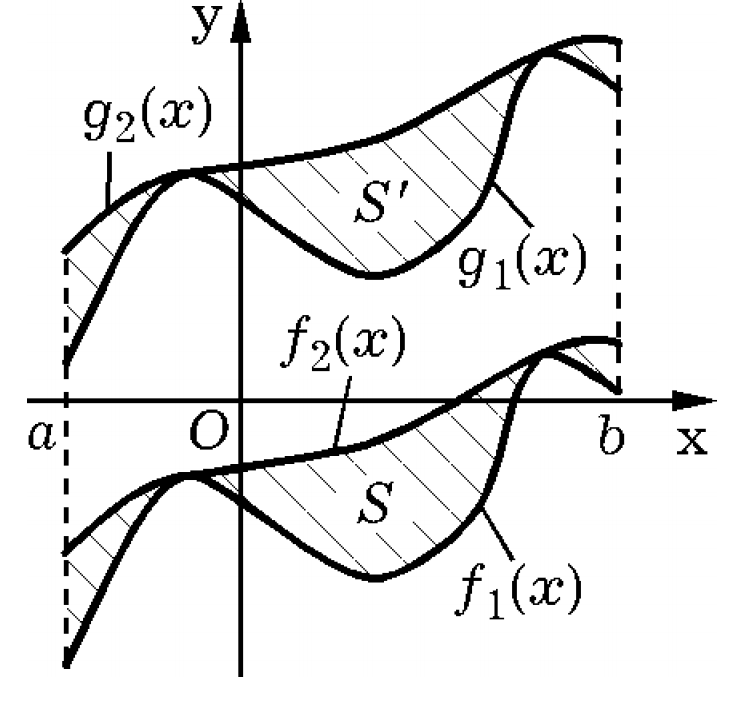
\includegraphics[scale=0.2]{pic15_1.png} \label{pic:15:1}\\
Рис. 2
\end{center}

Положим $g_2(x) = f_2(x) + M$. Тогда $g_2(x) \geqslant g_1(x)$ для любого $x \in [a,b]$. Заштрихованные на рис. \ref{pic:15:1} площади $S$ и $S'$ равны, так как одна получается из другой сдвигом, а при сдвиге площадь не меняется. Площадь $S'$ равна разности $S_2 - S_1$ площадей криволинейных трапеций: $S_2$ ограничена графиком функции $g_2(x)$, $S_1$ --- графиком функции $g_1(x)$. Используя геометрический смысл определенного интеграла как площади криволинейной трапеции и линейность интергала, получаем
\[ S = S' = S_2 - S_1 = \int_a^b (g_2(x) - g_1(x)) ~dx = \int_a^b (f_2(x) - f_1(x)) ~dx.\]
\end{proof}

\begin{remark} \label {rem:15:1}
Пусть плоская фигура ограничена кривой, заданой параметрически уравнениями $x = x(t),~y = y(t),~t \in [\alpha, \beta]$, и, может быть , вертикальными прямыми и осью $Ox$. Функция $y(t)$ непрерывна на отрезке $[\alpha, \beta]$, а $x(t)$ дифференцируема и имеет непрерывную на $[\alpha, \beta]$ производную. Кроме того, двигаясь по кривой в направлении роста $t$ фигура остается справа. Тогда площадь этой фигуры равна
\[ S = \int_{\alpha}^{\beta} y(t) x'(t)~dt.\]
\end{remark}

\begin{proof}
Разрежем рассматриваемую фигуру $\Phi$ вертикальными прямыми на фигуры $\Phi_i,~i = 1,\ldots, k$, рассмотренного в теореме \ref{th:15:1} вида. Кривая, ограничивающая фигуру $\Phi$, также разрежется на несколько ($m$) частей, которые заданы параметрически теми же уравнениями $x = x(t)$, $y = y(t)$, но с разной областью изменения параметра: $t \in [\alpha_j, \beta_j],~j = 1,\ldots, m$, при этом
\[\alpha = \alpha_1 < \beta_1 = \alpha_2 < \beta_2 = \alpha_3  < \ldots < \beta_m = \beta. \]

По теореме \ref{th:15:1} площадь $S_i$ части $\Phi_i$ равна интегралу от разности $f_{2i}(x) - f_{1i}(x)$ функций на некоторой части $[a_i, b_i]$ отрезка $[a, b]$, где $y = f_{2j}(x)$ --- уравнение верхней границы фигуры $\Phi_i$ а $y = f_{1i}(x)$ --- уравнение нижней границы. По условию эти границы заданы параметрически уравнениями $x = x(t)$, $y = y(t)$. Пусть $[\alpha_{j_i}, \beta_{j_i}]$ --- область изменения параметра на верхней границе, $[\alpha_{k_i}, \beta_{k_i}]$ --- область изменения параметра на нижней границе ($1 \leqslant j_i,~k_i \leqslant m$). Тогда образ и отрезка $[\alpha_{j_i}, \beta_{j_i}]$, и отрезка $[\alpha_{k_i}, \beta_{k_i}]$ при отображении $t \to x(t)$ есть отрезок $[a_i, b_i]$. При этом, так как ``двигаясь по кривой в направлении роста $t$ фигура остается справа'' (см. условие), то
\begin{equation} \label{eq:15:1}
x(a_{j_i}) = a_i,~~~x(\beta_{j_i}) = b_i,~~~x(\alpha_{k_i}) = b_i,~~~x(\beta_{k_i}) = a_i.
\end{equation}

Интеграл из теоремы \ref{th:15:1} для площади $S_i$ представим в виде разности двух интегралов и в каждом из них сделаем замену переменной $x = x(t)$, и получим
\[ S_i = \int_{a_i}^{b_i} f_{2i} (x) ~dx - \int_{a_i}^{b_i} f_{1i}(x)~dx = \int_{\alpha_{j_i}}^{\beta_{j_i}} y(t) x'(t)~dt - \int_{\beta_{k_i}}^{\alpha_{k_i}} y(t) x'(t)~dt,\]

где учтено \eqref{eq:15:1} и то, что $f_{2i} (x(t)) = y(t)$ при $t \in [\alpha_{j_i}, \beta_{j_i}]$ и $f_{1i}(x(t)) = y(t)$ при $t \in [\alpha_{k_i}, \beta_{k_i}]$. Меняя в последнем интеграле порядок интегрирования, получаем:
\[ S_i = \int_{\alpha_{j_i}}^{\beta_{j_i}} y(t) x'(t)~dt + \int_{\alpha_{k_i}}^{\beta_{k_i}} y(t) x'(t)~dt.\]

Отметим, что возможна ситуация, когда нижняя или верхняя граница фигуры $\Phi_i$ есть отрезок оси $Ox$. Тогда в выражении для площади $S_i$ присутствует только один из интегралов (второй равен нулю).\\

Плодащь $S$ всей фигуры $\Phi$ равна сумме площадей $S_i,~i = 1,\ldots,k$. Так как для любого $j = 1,\ldots,m$ уравнения $x= x(t),~y = y(t)$ при $t \in [\alpha_j, \beta_j]$ задают границу (нижнюю или верхнюю) в точности одного участка, то интеграл от функции $y(t) x'(t)$ на отрезке $[\alpha_j, \beta_j]$ встречается в сумме $\sum\limits_{i=1}^k S_i$ в точности один раз. Используя свойство аддитивности, преобразуем эту сумму интегралов в один интеграл. Получим утверждение данного следствия.
\end{proof}

\newpage \section{Вопрос №16} %%%%%%%%%%%%%%%%%%%%%%%%% Вопрос 16
\begin{framed}
Вывести формулу для вычисления с помощью определенного интеграла площади плоской
фигуры, граница которой задана в полярных координатах.
\end{framed}

\begin{lemma} \label{lemm:16:1}
Пусть функции $g$ и $F$ определены в окрестности точки $x$, $g$ непрерывна в $x$. Функция $G(\Delta x)$ определена в выколотой окрестности $\dot{U}(0)$ нуля и
\[ \forall \Delta x \in \dot{U}(0)~~~~ \inf_{t \in [x,x + \Delta x]}g(t) \leqslant \frac{\Delta F(x)}{G(\Delta x)} \leqslant \sup_{t \in[x,x + \Delta x]} g(t).\]
Если $G(\Delta x) = h \Delta x + o(\Delta x),~h \neq 0,$ то $F'(x) = g(x)h$.\\
\end{lemma}

\textbf{Метод дифференциалов:}
\begin{enumerate}
\item[1)] решаемую задачу переформулируют в задачу поиска значения $F(b)$ функции $F(x)$, определенной на отрезке $[a,b]$, причем $F(a) = 0$;
\item[2)] используя оценки для $\Delta F(x)$, лемму или другие подобные соображения, получают формулу $dF(x) = f(x)dx$;
\item[3)] из формулы \hyperref[th:11:1]{Ньютона --- Лейбница} выводят равенство $F(b) = \int_a^b f(x)~dx$.\\
\end{enumerate}

\begin{theorem}[Формула для площади в полярных координатах.] \label{th:16:1}
Пусть в полярных координатах ($\rho, \varphi$) плоская фигура $\Phi$ ограничена кривой $\rho = \rho(\varphi)$ и двумя лучами $\varphi = \alpha$ и $\varphi = \beta$, ($\alpha < \beta$). Функция $\rho(\varphi)$ непрерывна на отрезке $[\alpha, \beta]$. Тогда площадь фигуры $\Phi$ равна
\[ S = \frac{1}{2}\int_{\alpha}^{\beta} \rho^2(\varphi)~d\varphi.\]
\end{theorem}
\begin{proof}[Доказательство методом дифференциалов:] площадь фигуры, ограниченной кривой $\rho = \rho(\varphi)$ и лучами, составляющими с полярной осью углы $\alpha$ и $\beta > \alpha$, обозначим через $S(\varphi)$. Тогда $S(\alpha) = 0$, а $S(\beta)$ --- искомая плодащь. Фигура между лучами $\varphi$ и $\varphi + \Delta \varphi$ содержится в круговом секторе с углом $\Delta \varphi$ радиуса $\rho_M = \max\limits_{t \in [\varphi, \varphi + \Delta \varphi] }\rho(t)$ и содержит круговой сектор с тем же углом $\Delta \varphi$ радиуса $\rho_m = \min\limits_{t \in [\varphi, \varphi + \Delta \varphi]} \rho(t)$. Поэтому площадь $\Delta S$ этой фигуры удовлетворяет неравенствам
\[ \frac{1}{2} \rho^2_m \Delta \varphi \leqslant \Delta S \leqslant \frac{1}{2} \rho^2_M \Delta \varphi.\]
Полагая $F = S$, $h = 1$, $g = \frac{1}{2} \rho^2$, мы видим, что условия леммы выполняются, а значит, $dS = \frac{1}{2} \rho^2(\varphi)~d \varphi$. Интегрируя $dS$ от $\alpha$ до $\beta$ получаем указанную формулу.
\end{proof}

\newpage \section{Вопрос №17} %%%%%%%%%%%%%%%%%%%%%%%%% Вопрос 17
\begin{framed}
Привести формулу для вычисления с помощью определенного интеграла объема тела по площадям параллельных сечений в декартовой системе координат.
\end{framed}

\begin{theorem} \label{th:17:1}
Пусть тело заключено между плоскостями $x = a$ и $x = b$, а все сечения этого тела плоскостями, перпендикулярными координатной оси $Ox$, известны, причем зависимость $S(x)$ площади сечения от абсциссы $x \in [a,b]$ является заданной функцией, непрерывной на отрезке $[a,b]$. Тогда объем этого тело равен
\[ V = \int_a^b S(x)~dx.\]
\end{theorem}

\newpage \section{Вопрос №18} %%%%%%%%%%%%%%%%%%%%%%%%% Вопрос 18
\begin{framed}
Вывести формулу для вычисления с помощью определенного интеграла объемов тел вращения вокруг осей OX и OY в декартовой системе координат.
\end{framed}

\begin{theorem} \label{th:18:1}
Пусть фигура $\Phi$ --- криволинейная трапеция непрерывной и неотрицательной функции $f(x)$ на отрезке $[a,b]$. Тогда:
\begin{enumerate}
\item[a)] объем тела, образованного вращением фигуры $\Phi$ вокруг оси $Ox$ равен
\[ V_{Ox} = \pi \int_a^b f^2(x)~dx.\]
\item[б)] При $a \geqslant 0$ и вращении фигуры $\Phi$ вокруг оси $Oy$ получаем тело с объемом
\[ V_{Oy} = 2 \pi \int_a^b x f(x)~dx.\]
\end{enumerate}
\end{theorem}
\begin{proof}[Доказательство методом дифференциалов:]
~\\
\begin{enumerate}
\item[a)] Объем тела, образованного вращением воркуг оси $Ox$ криволинейной трапеции, ограниченной графиком функции $f$ на отрезке $[a,x]$, обозначим через $V(x)$. Тогда $V(a) = 0$, а $V(b)$ --- искомый объем. Приращение $\Delta V$ этой функции в точке $x$ есть объем части рассматриваемого тела между плоскостями с абциссами $x$ и $x + \Delta x$. Эта часть содержится и содержит круговые цилиндры ширины $\Delta x$ радиуса $f_M = \max\limits_{t \in [x, x + \Delta x]} f(t)$ и $f_m = \min\limits_{t \in [x, x + \Delta x]}f(t)$ соответственно, поэтому
\[ \pi f^2_m \Delta x \leqslant \Delta V \leqslant \pi f^2_M \Delta x.\]

Применяя лемму, когда $F = V$, $h = 1$, $g = \pi f^2$, получаем $dV = \pi f^2(x)~dx$ и указанную формулу для $V_{Ox}$.

\item[б)] Обозначим теперь через $V(x)$ обхем тела, образованого вращением вокруг оси $Oy$ той же криволинейной трапеции на отрезке  $[a,x]$. Две круговые цилиндрические поверхности радиуса $x$ и $x + \Delta x$ вырезают из рассматриваемого тела часть объемом $\Delta V$. Эта часть содержится и содержит цилиндрическую оболочку радиуса $x$, толщиной $\Delta x$ высотой  $f_M = \max\limits_{t \in [x, x + \Delta x]} f(t)$ и $f_m = \min\limits_{t \in [x, x + \Delta x]}f(t)$ соответственно. Объем цилиндрической оболочки радиуса $x$, толщиной $\Delta x$ и высотой $h$ равен $\pi (x + \Delta x)^2 h - \pi x^2 h = \pi h(2x \Delta x + \Delta x^2)$. Поэтому
\[ \pi f_m \leqslant \frac{\Delta V(x)}{2x \Delta x + \Delta x^2} \leqslant \pi f_M,\]

по лемме $dV = 2\pi x f(x)~dx$, и из формулы  \hyperref[th:11:1]{Ньютона --- Лейбница} следует утверждение б) теоремы.
\end{enumerate}
\end{proof}

\newpage \section{Вопрос №19} %%%%%%%%%%%%%%%%%%%%%%%%%% Вопрос 19
\begin{framed}
Дать определения длины дуги кривой и спрямляемых кривых. Доказать достаточное условие спрямляемости кривых.
\end{framed}

\textbf{Длиной} $L(\gamma)$ называется точная верхняя грань длин ломаных, вписанных в кривую $\gamma$. Кривая называется \textbf{спрямляемой}, если ее длина существует и конечна.

\begin{theorem}[Достаточное условие спрямляемости кривой] \label{th:19:1}
Гладкая кривая спрямляема. Длина $L(\gamma)$ гладкой кривой $\gamma$ с параметризацией $\vec{r} = (x_1(t),\ldots,x_m(t)),~t\in[a,b],\\a < b$, вычисляется по формуле
\[ L(\gamma) = \int_a^b |\pvec{r}'(t)|~dt = \int_a^b \sqrt{\sum_{i=1}^m (x_i'(t))^2}~dt.\]
\end{theorem}

Докажем сначала обобщение на векторный случай теоремы об оценке модуля интеграла. При этом определенный интеграл от векторной функции будем понимать как вектор, состоящий из определенных интегралов от ее координатных функций.

\begin{lemma}[оценка модуля интеграла векторной функции] \label{lemm:19:1}
Для непрерывной на отрезке $[a,b]$, $a < b$, векторной функции $\vec{r}(t)$ справедливо неравенство
\[ \left| \int_a^b \vec{r}(t)~dt \right| \leqslant \int_a^b |\vec{r}(t)|~dt.\]
\end{lemma}
\begin{proof}[Доказательство леммы] Пусть $x_1(t),\ldots,x_m(t)$ --- координатные функции вектор-функции $\vec{r}(t)$. По условию векторная функция $\vec{r}(t)$ непрерывна на отрезке $[a,b]$, а значит, непрерывны функции $x_1(t), \ldots, x_m(t)$ и $|\vec{r}(t)|$. Поэтому определены и конечны все интегралы леммы, а значит, соответствующие интегральные суммы не зависят от выбора разбиений, и для доказательства неравенства леммы мы можем учитывать только равномерные разбиения отрезка. Разделим отрезок $[a,b]$ на $n$ равных частей и положим $t_j = a + \frac{b-a}{n}j$, $j = 0,1,\ldots,n$. Преобразуя суммы и используя неравество Коши --- Буняковского, получаем
\[
\begin{aligned}
\sum_{i=1}^m \left( \sum_{j=1}^n x_i(t_j) \right)^2&= \sum_{i=1}^m\left( \sum_{j_1 = 1}^n x_i (t_{j_1}) \right) \left( \sum_{j_2 = 1}^n x_i (t_{j_2}) \right) =\\
&= \sum_{j_1 = 1}^n \sum_{j_2 = 1}^n \left( \sum_{i=1}^m x_i (t_{j_1}) x_i (t_{j_2}) \right) \leqslant\\
&\leqslant \sum_{j_1 = 1}^n \sum_{j_2 = 1}^n \sqrt{\sum_{i=1}^m x_i^2 (t_{j_1})} \sqrt{\sum_{i=1}^m x_i^2 (t_{j_2})} = \left( \sum_{j=1}^n \sqrt{\sum_{i=1}^m x_i^2 (t_j)}\right).
\end{aligned}\]

Таким образом, интегральные суммы для функций $x_1(t), \ldots, x_m(t)$ и $|\vec{r}(t)|$, соответствующие разбиению $P = (t_0, \ldots, t_n)$ с отмеченными точками $\xi_1 = t_1, \ldots, \xi_n = t_n$ отрезка $[a,b]$, связаны неравенством
\[\sum_{i=1}^m \sigma(x_i; P, \xi)^2 = \sum_{i=1}^m \left( \sum_{j=1}^n x_i (t_j) \frac{b-a}{n}\right)^2 \leqslant \left( \sum_{j=1}^n \sqrt{\sum_{i=1}^m x_i^2 (t_j)} \frac{b-a}{n}\right)^2 = \sigma(|\vec{r}|; P, \xi)^2.\]

Переходя в этом неравенстве к пределу $\lambda \to 0$ (в данном случае это означает $n \to \infty$), получаем утверждение леммы.
\end{proof}

\begin{proof} [Доказательство теоремы \ref{th:19:1}]
Рассмотрим произвольное разбиение $P = (t_0, \ldots, t_n)$ отрезка $[a,b]$ и соответствующую ломаную $\vec{r}(t_0) \vec{r}(t_1) \ldots \vec{r}(t_m)$, вписанную в кривую $\gamma$. Для длины $L_P$ этой ломанной, используя формулу Ньютона --- Лейбница, лемму и аддитивность интеграла, получаем
\[ L_P = \sum_{i=1}^n | \vec{r}(t_i) - \vec{r} (t_{i - 1})| = \sum_{i=1}^n \left| \int_{t_{i-1}}^{t_i} \pvec{r}'(t)~dt \right| \leqslant \sum_{i=1}^n \int_{t_{i-1}}^{t_i} | \pvec{r}'(t)| ~dt = \int_a^b |\pvec{r}'(t)|~dt.\]

Таким образом, длина любой ломанной, вписанной в кривую $\gamma$, ограничена сверху указанным интегралом. По теореме о точных гранях существует и конечна точная верхняя грань длин таких ломаных. А значит, кривая $\gamma$ спрямляема, а ее длина удовлетворяет неравенству
\[ L(\gamma) = \sup_{P}L_P \leqslant \int_a^b |\pvec{r}'(t)|~dt.\]

Для доказательства равенства рассмотрим произвольное $\varepsilon > 0$. Так как производная векторной функции $\pvec{r}'(t)$ непрерывна на отрезке $[a,b]$, то непрерывны на этом отрезке производные $x_1'(t), \ldots, x_m'(t)$ ее координатных функций. По теореме Кантора эти функции равномерно непрерывны на отрезке $[a,b]$, значит, найдется такое число $\delta > 0$, что $|\pvec{r}'(t) - \pvec{r}'(s)| \leqslant \sum\limits_{j=1}^m |x_j'(t) - x_j'(s)| < \varepsilon$, если $|t - s| < \delta$. Пусть параметр разбиения $P$ меньше $\delta$. Если $t_{i-1} \leqslant t \leqslant t_i$, то $|t - t_i| < \delta$ и поэтому
\[ |\pvec{r}'(t)| = |\pvec{r}'(t_i) + \pvec{r}'(t) - \pvec{r}'(t_i) | \leqslant |\pvec{r}'(t_i)| + |\pvec{r}'(t) - \pvec{r}'(t_i)| < |\pvec{r}'(t_i)| + \varepsilon.\]

Из доказанного неравенства и свойства монотонности интеграла получаем
\[ \int_{t_{i-1}}^{t_i} |\pvec{r}'(t)|~dt - \varepsilon \Delta t_i \leqslant \int_{t_{i-1}}^{t_i} (|\pvec{r}'(t_i)| + \varepsilon)~dt - \varepsilon \Delta t_i = |\pvec{r}'(t_i)| \Delta t_i.\]

Используя свойства интеграла, неравенство треугольника, лемму и доказанное ранее неравенство $|\pvec{r}'(t_i) - \pvec{r}'(t)| < \varepsilon$, получаем
\[ |\pvec{r}'(t_i)| \Delta t_i = \left| \int_{t_{i-1}}^{t_i} \pvec{r}'(t_i)~dt \right| = \left| \int_{t_{i-1}}^{t_i} \pvec{r}'(t)~dt  + \int_{t_{i-1}}^{t_i} (\pvec{r}'(t_i) - \pvec{r}'(t))~dt \right| \leqslant \left| \int_{t_{i-1}}^{t_i} \pvec{r}'(t)~dt \right| +\]
\[+ \left| \int_{t_{i-1}}^{t_i} (\pvec{r}'(t_i) - \pvec{r}'(t))~dt \right| \leqslant \left\lvert \pvec{r}(t)\bigr\vert_{t_{i-1}}^{t_i} \right\rvert  + \int_{t_{i-1}}^{t_i} |\pvec{r}'(t_i) - \pvec{r}'(t)| ~dt \leqslant |\pvec{r}(t_i) - \pvec{r}(t_{i-1}) | + \varepsilon \Delta t_i.\]

Суммируя доказанные неравенства по $i = 1, \ldots, n$, получаем
\[\int_a^b |\pvec{r}' (t)| ~dt = \sum_{i=1}^n \int_{t_{i-1}}^{t_i} |\pvec{r}'(t)| ~dt \leqslant \sum_{i=1}^n |\pvec{r}(t_i) - \pvec{r}(t_{i-1}) | + 2 \varepsilon \sum_{i=1}^n \Delta t_i \leqslant L(\gamma) + 2 \varepsilon (b-a).\]

Ввиду произвольности $\varepsilon$ отсюда следует, что $\int_a^b |\pvec{r}'(t)|dt \leqslant L(\gamma)$, и это завершает доказательство теоремы.
\end{proof}

\newpage \section{Вопрос №20} %%%%%%%%%%%%%%%%%%%%%%% Вопрос 20
\begin{framed}
Определение длины дуги кривой. Вывести формулы для вычисления с помощью определенного интеграла длины дуги кривой, заданой параметрически, в декартовой или полярной системах координат.
\end{framed}

\textbf{Длиной} $L(\gamma)$ называется точная верхняя грань длин ломаных, вписанных в кривую $\gamma$. Кривая называется спрямляемой, если ее длина существует и конечна.\\

Пусть $k$ --- натуральное число. Функцию $f$, определенную на множестве  $A \subseteq \mathbb{R}$, называют $k$ \textbf{раз непрерывно дифференцируемой на множестве} A, если в каждой точке $x \in A$ существует ее производная $f^{(k)} (x)$ порядка $k$, которая непрерывна на множестве $A$. В случае $k = 1$ таую функцию называют \textbf{непрерывно диффернцируемой}, в случае $k = 2$ --- \textbf{дважды непрерывно дифференцируемой}. Множество всех $k$ раз непрерыно дифференцируемых на множестве $A$ функций обозначают $C^k A$.

\begin{theorem} \label{th:20:1}
~
\begin{enumerate}
\item[а)] Если функции $x(t)$ и $y(t)$ непрерывно дифференцируемы на отрезке $[a,b]$, то плоская кривая, заданная параметрически уравениями $x = x(t),~y = y(t),~t\in [a,b]$, имеет длину
\[ \int_a^b \sqrt{(x'(t))^2 + (y'(t))^2}~dt.\]

\item[б)] Длина графика непрерывно дифференцируемой на отрезке $[a,b]$ функции $f(x)$ равна
\[ \int_a^b \sqrt{1 + (f'(x))^2}~dx.\]

\item[в)] Если функция $\rho(\varphi)$ непрерывно дифференцируема на отрезке $[\alpha, \beta]$, то длина кривой, заданной в полярной системе координат $(\varphi, \rho)$ ураенением $\rho = \rho(\varphi)$ равна
\[ \int_{\alpha}^{\beta} \sqrt{(\rho(\varphi))^2 + (\rho'(\varphi))^2}~d\varphi.\]
\end{enumerate}

\begin{proof}
Утверждение а) следует из теоремы \ref{th:19:1} в случае $m = 2$. Полагая $x = t,~y = f(t)$ получаем утверждение б). В полярных координатах, считая $\varphi$ параметром, имеем параметризацию $x(\varphi) = \rho(\varphi),~ y(\varphi) = \rho(\varphi)\sin \varphi$ кривой. Так как
\[ x'(\varphi) = \rho'(\varphi)\cos\varphi - \rho(\varphi)\sin\varphi,~~ y'(\varphi) = \rho'(\varphi)\sin\varphi + \rho(\varphi)\cos\varphi,\]

то $(x'(\varphi))^2 + (y'(\varphi))^2 = (\rho(\varphi))^2 + (\rho'(\varphi))^2$. А значит, из а) получаем в).
\end{proof}
\end{theorem}


\newpage \section{Вопрос №21} %%%%%%%%%%%%%%%%%%%%%%%%%%% Вопрос 21
\begin{framed}
Кривизна кривой и ее геометрический смысл. Вывести формулы для вычисления кривизны графика функции и кривизны плоской кривой, заданной параметрически.
\end{framed}

Угол $\theta$ между касательными к кривой в точках $M$ и $N$ называется \textbf{углом смежности} дуги $\arc{MN}$. Если две дуги $\arc{MN}$ и $\arc{M'N'}$ имеют одинаковую длину $(L(\arc{MN}) = L(\arc{M'N'}))$ и угол смежности первой дуги больше угла смежности второй дуги $\theta > \theta'$, то первая дуги искривелна сильнее второй дуги. Таким боразом, угол сежности характеризует искривленность дуги при условии постоянства ее длины. Поэтому воодят понятие \textbf{средней кривизны дуги} как отношение угла смежности дуги к ее длине: $k_{\text{ср.}} = \dfrac{\theta}{L(\arc{MN})}$, а \textbf{кривизной дуги} $\gamma$ в точке $M_0$ называют неотрицательное число $k$, равное пределу средней кривинзны $\dfrac{\theta}{L(\arc{M_0M})}$ дуги $\arc{M_0 M}$ при стремлении точки $M$ к точке $M_0$, при этом точка $M$ остается на кривой $\gamma$.

\begin{theorem} \label{th:21:1}
Кривизна кривой в $\mathbb{R}^3$, заданной дважды непрерывно дифференцируемой векторной функнией $\pvec{r}'(t)$, в регулярной точке $\pvec{r}(t_0)$ $(|\pvec{r}'(t_0)| \neq 0)$ вычисляется по формуле
\[ k = \frac{|\pvec{r}'(t_0) \times \pvec{r}''(t_0)|}{|\pvec{r}'(t_0)|^3}.\]
\end{theorem}
\begin{proof}
Пусть $M_0 = \pvec{r}(t_0)$, $M = \pvec{r}(t)$ --- точки кривой, $M_0$ --- регулярная точкк, $\theta$ --- угол смежности дуги $\arc{M_0M}$, $\Delta t = t - t_0$. В виду неравенства $|\pvec{r}'(t_0)| \neq 0$ и непрерывности $\pvec{r}'$ при малых отклонениях $\Delta t$ имеем также $|\pvec{r}'(t)| \neq 0$. Из определения $\theta$, геометрического смысла производной, формулы Тейлора для $\pvec{r}'(t)$ и свойств векторного произведения получаем
\[
\begin{aligned}
 \sin\theta = \frac{|\pvec{r}'(t_0) \times \pvec{r}'(t)|}{|\pvec{r}'(t_0)||\pvec{r}'(t)|} &= \frac{|\pvec{r}'(t_0) \times (\pvec{r}'(t_0) + \Delta t \pvec{r}''(t_0) + o(\Delta t))|}{|\pvec{r}'(t_0)||\pvec{r}'(t)|} =\\
&= |\Delta t| \frac{|\pvec{r}'(t_0) \times \pvec{r}''(t_0)|}{|\pvec{r}'(t_0)||\pvec{r}'(t)|} + o (\Delta t).
\end{aligned}
\]
Отсюда, го первого замечательного предела и непрерывности $\pvec{r}'(t)$ следует
\[ \lim_{\Delta t \to 0} = \lim_{\Delta t \to 0} \frac{\theta}{\sin \theta} \lim_{\Delta t \to 0}\frac{\sin \theta}{|\Delta t|} = \lim_{\Delta t \to 0} \left( \frac{|\pvec{r}'(t_0) \times \pvec{r}''(t_0)|}{|\pvec{r}'(t_0)||\pvec{r}'(t)|} + \frac{o (\Delta t)}{|\Delta t|}\right) = \frac{|\pvec{r}'(t_0) \times \pvec{r}''(t_0)|}{|\pvec{r}'(t_0)|^2.}\]
Наконец, из определения кривизны и формулы для длины кривой получаем
\[ k = \lim_{M \to M_0} \frac{\theta}{L(\arc{M_0 M})} = \lim_{\Delta \to 0} \frac{\theta}{|\Delta t|} \lim_{\Delta t \to 0}\frac{|\Delta t|}{L(\arc{M_0 M})} = \frac{|\pvec{r}'(t_0) \times \pvec{r}''(t_0)|}{|\pvec{r}'(t_0)|^2}\frac{1}{|\pvec{r}'(t_0)|}.\]
\end{proof}

\begin{theorem}[Кривизна графика функции] \label{th:21:2}
Если функция $y = f(x)$ дважды непрерывно дифференцируема в точке $x$, то кривизна графика этой функции в точке $(x, f(x))$ равна
\[ k(x) = \frac{|f''(x)|}{\left( 1 + (f'(x))^2 \right)^{3/2}}.\]
\end{theorem}

\begin{proof}
Считая $x$ параметром, представим кривую $y = f(x)$ векторной функцией $\pvec{r}(x) = x \pvec{i} + f(x) \pvec{j}$. Тогда $\pvec{r}'(x) = \pvec{i} + f'(x) \pvec{j},~\pvec{r}''(x) = f''(x)\pvec{j}$,
\[ |\pvec{r}'(x) \times \pvec{r}''(x)| = |f''(x) \pvec{i} \times \pvec{j}| = |f''(x)|,~~ |\pvec{r}'(x)| = \sqrt{1 + (f'(x))^2},\]
и из теоремы \ref{th:21:1} следует данная теорема.
\end{proof}

\newpage \section{Вопрос №22} %%%%%%%%%%%%%%%%%%%%%%%%%%%%%% Вопрос 22
\begin{framed}
Определение радиуса кривизны, круга кривизны и центра кривизны плоской кривой. Эволюта и эвольвента. Механический способ построения по заданной кривой одной из ее эвольвент. Доказать геометрический смысл круга кривизны. Вывести формулу для вычисления
координат центра кривизны.
\end{framed}

Пусть $k$ --- кривизна плоской кривой $\gamma$ в точке $M_0 \in \gamma$. Величину $R = 1 / k$, обратную кривизне называют \textbf{радиусов кривизны кривой $\gamma$ в точке $M_0$}. Если $k = 0$, то радиус $R$ кривизны кривой полагают равным $+\infty$.\\

Пусть плоская кривая $\gamma$ имеет ненулевую кривизну в точке $M_0$. Выберем на плоскости такую систему координат, в которой $\gamma$ задается уравнением $y = f(x)$, а $x_0$ --- абцисса точки $M_0$. Тогда из теоремы \ref{th:21:2} следует, что $f''(x_0) \neq 0$, т.е. точка $M_0$ есть точка выпулости (вогнутости) кривой $\gamma$, а значит, в окрестности $M_0$ кривая лежит по подну сторону от касательной. Рассмотрим нормаль к кривой $\gamma$ в точке $M_0$. Точку $C_0$ нормали, расположенной на расстоянии радиуса кривизны от точки $M_0$ в сторону вогнутости кривой называют \textbf{центром кривизны кривой в точке $M_0$}, а круг (окружность) с центром в $C_0$, радиус которого (которой) равен радиусу кривизны, называют \textbf{кругом (окружностью) кривизны кривой в точке $M_0$}.\\

Множество центров кривизны кривой называют ее \textbf{эволютой}. По отношению к своей эволюте кривую называют \textbf{эвольвентой} (иногда \textbf{инволютой} или \textbf{разверткой}).

\begin{theorem} [Геометрический смысл окружности кривизны] \label{th:22:1}
Окружность кривизны плоской гладкой кривой $\gamma \in C^2$ в точке $M$ --- это единственная окружность, которая касается кривой в точке $M$ с порядком 2, т.е.
\[ \lim_{x \to x_0} \frac{|f(x) - g(x)|}{|x - x_0|^2} = 0,\] 
где $f(x)$ и $g(x)$ --- функции, графики которых в окрестности точки $x_0$ совпадают с кривой и окружностью соответственно, $x_0$ --- абсцисса точки M.
\end{theorem}
\begin{proof}
Следует из формулы Тейлора для функций $f(x)$ и $g(x)$ в точке $x_0$. Действительно, из определений следует, что кривая $\gamma$ и ее окружность кривизны имеют одинаковые касательные, впуклось и кривизну. Поэтому $f'(x_0) = g'(x_0)$, так как сопадают касательные к графикам этих функций. Производные $f''(x_0)$ и $g''(x_0)$ имеют одинаковые знаки, поскольку выпуклось этих функйий совпадает. Наконец, из формулы для кривизны теоремы \ref{th:21:1}, равенства кривизн и первых производный функций $f$ и $g$ в точке $x_0$ получаем равенство $|f''(x_0)| = |g''(x_0)|$. Таким образом, многочлены Тейлора порядка 2 для функций $f(x)$ и $g(x)$ в точке $x_0$ совпадают. Из формулы Тейлора с остаточным членом в форме Пеано получаем $f(x) - g(x) = 0(|x- x_0|^2))$, а значит, графики функций $f(x)$ и $g(x)$ касаются в точке $M$ с порядком 2.\\

Единственность указанной окружности следует из того, что любая окружность однозначно определяется касательной в заданной точке, направлением выпуклости и кривизной (радиусом).
\end{proof}

\begin{theorem}[Координаты центра кривизны]
Если функция $f(x)$ дважды непрерывно дифференцируема в окрестности точки $x_0$, и $f''(x_0) \neq 0$, то координаты $\xi, \eta$ центра кривизны графика этой функции в точке $(x_0,y_0 = f(x_0))$ равны
\begin{equation} \label{eq:22:1}
\xi = x_0 - f'(x_0) \frac{1 + (f'(x_0))^2}{f''(x_0)}~~~~\text{и}~~~~\eta = y_0 + \frac{1 + (f'(x_0))^2}{f''(x_0)}.
\end{equation}
\end{theorem}

\begin{proof}
Из теооремы \ref{th:21:2} и неравенства $f''(x_0) \neq 0$ следует, что $k(x_0) \neq 0$, а значит, центр $C_0$ кривизны кривой $y = f(x)$ в точке $M_0(x_0,y_0)$ определен. При $f'(x_0) \neq 0$ уравнение нормали к этой кривой в точке $M_0$ (\hyperref[pic:22:1]{рис. 3}) имеет вид
\[ y_{\text{Н}} = y_0 - \frac{x_{\text{Н}} - x_0}{f'(x_0)}, \]
где $x_{\text{Н}}$ и $y_{\text{Н}}$ --- координаты произвольной точки нормали. Поскольку центр $C_0$ кривизны лежит на нормали, то его координаты $\xi$ и $\eta$ тоже должны удовлетворять этому уравнению, т.е.
\begin{equation} \label{eq:22:2}
\eta = y_0 - \frac{\xi - x_0}{f'(x_0)}.
\end{equation}

\begin{center}
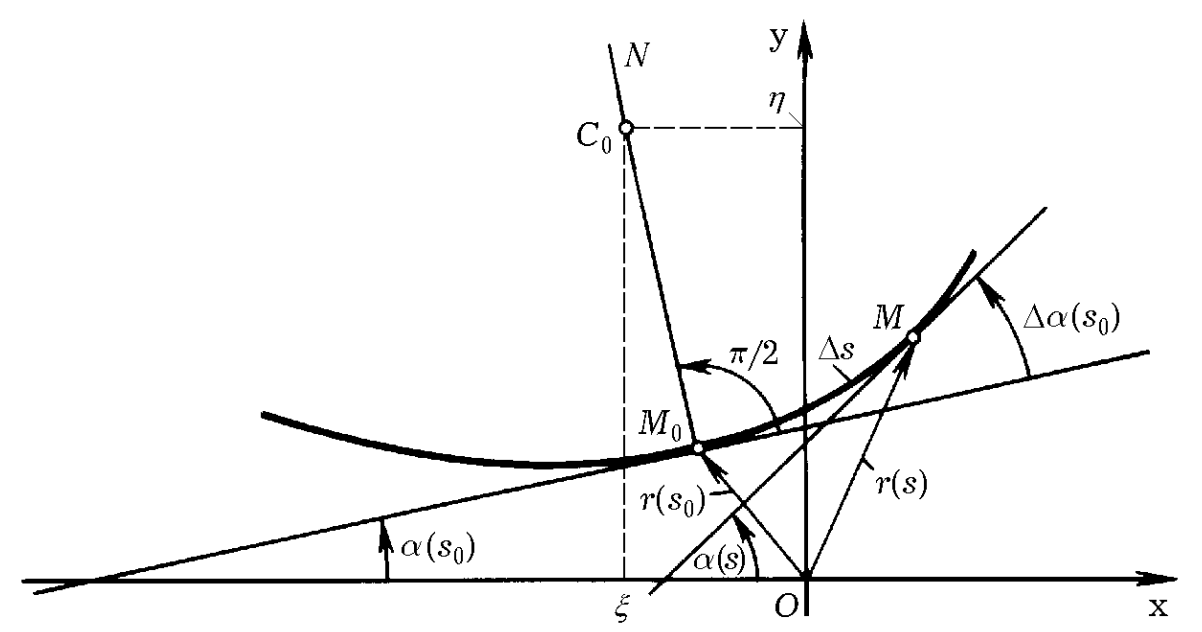
\includegraphics[scale=0.3]{pic22_1.png} \label{pic:22:1}\\
Рис. 3
\end{center}
В силу определения центра кривизны расстояние между точками $M_0(x_0, y_0)$ и $C_0(\xi, \eta)$ равно радиусу кривизны $R(x_0) = \dfrac{1}{k(x_0)}$. Поэтому
\begin{equation} \label{eq:22:3}
\sqrt{(\xi - x_0)^2 + (\eta + y_0)^2} = \frac{1}{k(x_0)}.
\end{equation}
Из \eqref{eq:22:2} следует $\xi - x_0 = -(\eta - y_0) f'(x_0)$. Подставляя это выражение и формулу для $k(x_0)$ из теремы \ref{th:21:2} в \eqref{eq:22:3}, находим
\[ \sqrt{(\eta - y_0)^2 (f'(x_0))^2 + (\eta - y_0)^2} = \frac{\left( 1 + (f'(x_0))^2\right)^{3/2}}{|f''(x_0)|}.\]
Отсюда
\begin{equation} \label{eq:22:4}
|\eta - y_0| = \frac{1 + (f'(x_0))^2}{|f''(x_0)|}.
\end{equation}
Если $f''(x_0) > 0$, то функция $f(x)$ строго выпукла вниз. В этом случае $\eta > y_0$ (см. \hyperref[pic:22:1]{рис. 3}) и поскольку $|f''(x_0)| = f''(x_0)$, то
\[ \eta - y_0 = \frac{1 + (f'(x_0))^2}{f''(x_0)},~~~\xi - x_0 = -f'(x_0)\frac{1 + (f'(x_0))^2}{f''(x_0)}.\]
Итак, при $f''(x_0) > 0$ формулы для координат центра кривизны имеют вид \eqref{eq:22:1}.\\

Если $f''(x_0) < 0$, то функция $f(x)$ строго выпукла вверх, и поэтому $\eta < y_0$. Т.е. и в этом случае модули в \eqref{eq:22:4} можно убрать, а значит, получить ту же самую формулу \eqref{eq:22:1}.\\

Если $f'(x_0) = 0$, т.е. касательноая к кривой горизонтальна, то $k(x_0) = |f''(x_0)|$, нормаль вертикальна и \eqref{eq:22:1} остается в силе: $\xi = x_0$ и $\eta = f(x_0) + 1 / f''(x_0)$.
\end{proof}

Отметим, что случай $f''(x_0) = 0$ соответстсует точке перегиба, в которой радиус кривизны, а значит, $\xi$ и $\eta$ бесконечны.

\begin{theorem}[свойства эволюты] \label{th:22:3}
\begin{enumerate}
\item[]
\item[(1)] Нормаль к кривой Г является касательной к ее эволюте $\Omega$ в соответствующем центре кривизны (см. \hyperref[pic:22:2]{рис. 4}).
\item[(2)] При строго монотонгном изменении радиуса $R$ кривизны кривой Г его криращение $\Delta R$ при перемещении центра кривизны данной кривой по дуге ее эволюты $\Omega$ равно по абсолютноему значению длине этой эволюты.
\end{enumerate}
\begin{center}
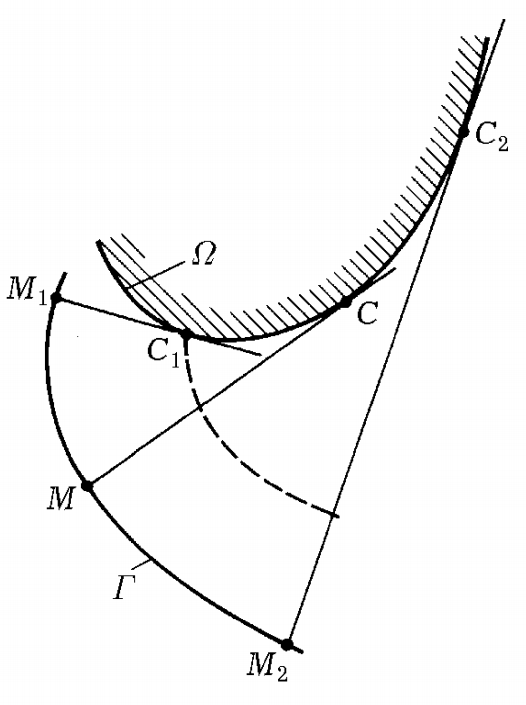
\includegraphics[scale=0.3]{pic22_2.png} \label{pic:22:2}\\
Рис. 4
\end{center}
\end{theorem}

Из теоремы \ref{th:22:3} следует \textbf{механический способ построения по заданной кривой одной из ее эвольвент}. А именно, если нерастяжимую нить, натянутую на жесткий контур, соответствующий заданной кривой $\Omega$ с дугой $C_1 C_2$ (см. \hyperref[pic:22:2]{рис. 4}), сматывать с этого контура, оставляя ее натянутой, то конец нити опишет дугу $M_1 M_2$ эвольвенты Г заданной кривой.

\newpage \section{Вопрос №23} %%%%%%%%%%%%%%%%%%%%%%%%% Вопрос 23
\begin{framed}
Дать определение несобственного интеграла от непрерывной функции на бесконечном промежутке. Доказать признаки сравнения для таких интегралов.
\end{framed}

Необходимым условием существования определенного итеграла является ограниченность подынтегральной функции и конечность отрезка интегрирования. Однако при рассмотрении теоретических вопросов и решении прикладных задач нередко появляется необходимость использовать при интегрировании неограниченные функции и бесконечные промежутки. Возникающие при этом интегралы принято называть \textbf{несобственными}.\\

Пусть функция $f(x)$ определена на бесконечном полуинтервале $[a, +\infty)$ и интрегрируема на любом кончном отрезке $[a,b] \subset [a, + \infty)$. Тогда для любого значения $b \in [a, + \infty)$ существует функция
\[ \Phi(b) = \int_a^b f(x)~dx~~~~~(a \leqslant b < + \infty).\]
Предел функции $\Phi(b)$ при $b \to + \infty$ называют \textbf{несобственный интегралом} от функции $f(x)$ \textbf{по бесконечному промежутку} $[a, + \infty)$ (или \textbf{несобственным интегралом первого рода}) и обозначают $\int_a^{+ \infty} f(x)dx$.

\begin{theorem}[свойства несобственных интегралов] \label{th:23:1}
\begin{enumerate}
\item[] % holy mother of crutches
\item[а)] Пусть сходятся несобственные интегралы от функций $f$ и $g$ по бесконечному промежутку $[a,+\infty)$, а $\lambda, \mu \in \mathbb{R}$. Тогданесобственный интеграл от функции $\lambda f + \mu g$ по промежутку $[a,+\infty)$ также сходится и 
\[ \int_a^{+\infty} (\lambda f + \mu g) ~dx = \lambda \int_a^{+\infty} f(x)~dx + \mu \int_a^{+\infty}g(x)~dx~~~\text{(\textbf{линейность})}.\]
\item[б)] Пусть функция $f(x)$ интегрируема на любом конечном отрезке $[a,b] \subset [a, +\infty)$, а $c > a$. Тогда несобственные интегралы от функции $f$ по промежуткам $[a, +\infty)$ и $[c, +\infty)$ либо оба сходятся, либо оба расходятся. И в случае их сходимости верно равенство
\[ \int_a^{+\infty} f(x)~dx = \int_a^c f(x)~dx + \int_c^{+\infty} f(x)~dx~~~\text{(\textbf{аддитивность})}.\]

% в теореме есть ещё 2 пунтка (Ньютон-Лейбниц и инт-ие по частям, но они не используются в доказательстве, так что опущены)

\end{enumerate}
\end{theorem}

\begin{proof}
Следует из определений и соответствующих свойств определенного интеграла.
\end{proof}

\begin{theorem} [признак сравнения 1]\label{th:23:2}
Пусть функции $f(x)$ и $g(x)$ интегрируемы на любом отрезке $[a,b] \subset [a, +\infty)$, причем $\exists c > a~\forall x \in [c, +\infty)~~ 0 \leqslant f(x) \leqslant g(x)$. Тогда  если сходится несобственный интеграл $\int_a^{+\infty}g(x)dx$, то сходится и интеграл $\int_a^{+\infty}f(x)dx$, а если расходится несобственный интеграл $\int_a^{+\infty}f(x)dx$, то расходится и $\int_a^{+\infty}g(x)dx$.
\end{theorem}

\begin{proof}
Пусть сходится интеграл $\int_a^{+\infty}g(x)dx$, тогда из свойства аддитивности несобственных интегралов сходится интеграл $\int_c^{+\infty}g(x)dx$. В силу определения это означает, что существует конечный предел
\[ \lim_{b \to +\infty}\int_c^b g(x)dx = M.\]
Поскольку по условию теоремы $g(x) \geqslant 0~\forall x \in [c, +\infty)$, то
\[ \forall d \in [c, +\infty)~~~ \int_d^{+\infty} g(x)~dx = \lim_{b \to +\infty} \int_d^b g(x)~dx \geqslant 0\]
как предел от неотрицательной функции. Еще раз используя свойство аддитивности, получаем
\[ \forall d \in [c, +\infty)~~~ \int_c^d g(x)~dx = \int_c^{+\infty} g(x)~dx - \int_d^{+\infty} g(x)~dx \leqslant M.\]
В соответствии с условием теоремы и свойством монотонности определенного интеграла
\[ \forall b \in [c, +\infty)~~~ 0 \leqslant \int_c^b f(x)~dx \leqslant \int_c^b g(x)~dx \leqslant M.\]
Так как $f(x) \geqslant 0~\forall x \in [c,+\infty)$, то фукнция $\Phi(b) = \int_c^b f(x)dx$ монотонно возрастает и ограничена сверху значением $M$. Следовательно, такая функция имеет предел, причем
\[ \lim_{b \to +\infty} \Phi(b) = \lim_{b \to +\infty} \int_a^b f(x)~dx \leqslant M, \]
что означает сходимость несобственного интеграла $\int_c^{+\infty}f(x)dx$, а значит, и $\int_a^{+\infty}f(x)dx$.
\end{proof}

\begin{theorem} [предельный признак сравнения] \label{th:23:3}
Пусть $f$, $g \in \mathcal{R}[a,b]~\forall b \in [a, + \infty)$, функция $f(x)$ неотрицательна, а $g(x)$ положительна при $x \geqslant c$ для некоторого $c \geqslant a$. Если существеует конечный ненулевой предел
\[ \lim_{x \to + \infty} \frac{f(x)}{g(x)} = \lambda \neq 0,\]
то несобственные интегралы $\int_a^{+ \infty} f(x)dx$ и $\int_a^{+ \infty} g(x)dx$ либо оба сходятся, либо оба расходятся.
\end{theorem}
\begin{proof}
 В силу определения предела функции для любого $\varepsilon > 0$ найдется такое  число $d > c$, что справедливо неравенство
\begin{equation} \label {eq:23:1}
(\lambda - \varepsilon) g(x) < f(x) < (\lambda + \varepsilon) g(x)~~~~~~\forall x > d.
\end{equation}
Выберем $\varepsilon$ так, чтобы было выполнено условие $\lambda - \varepsilon > 0$. Если сходится интеграл $\int_a^{+\infty}g(x)dx$, то в силу линейности сходится и интеграл $\int_a^{+\infty}(\lambda + \varepsilon) g(x)dx$, а тогда, согласно \eqref{eq:23:1} и теореме \ref{th:23:2} будет сходиться и интеграл от $f(x)$.\\

Если же сходится интеграл от $f(x)$, то в силу \eqref{eq:23:1} и теоремы \ref{th:23:2} сходится и интеграл от $(\lambda - \varepsilon)g(x)$, а тогда, согласно линейности будет сходиться и интеграл от $g(x)$.
\end{proof}

\newpage \section{Вопрос №24} %%%%%%%%%%%%%%%%%%%%%%%%%%%% Вопрос 24
\begin{framed}
Дать определение несобственного интеграла от неограниченной функции на конечном отрезке интегрирования. Сведение несобственного интеграла от неограниченной функции к несобственному интегралу по бесконечному промежутку. Сформулировать  признаки сходимости интегралов от неограниченной функции.
\end{framed}

Необходимым условием существования определенного интеграла является ограниченность подынтегральной функции и конечность отрезка интегрирования. Однако при рассмотрении теоретических вопросов и решении прикладных задач нередко появляется необходимость использовать при интегрировании неограниченные функции и бесконечные промежутки. Возникающие при этом интегралы принято называть \textbf{несобственными}.\\

Пусть функция $f(x)$ определена в полуинтервале $[a,b)$, неограничена при $x \to b-$ (это значит, что функция не является ограниченной ни в какой окрестности точки $b$, где точка $b$ может быть как конечной, так и бесконечной), но интегрируема на любом отрезке $[a,\eta] \subset [a,b)$. Тогда для любого $\eta \in [a,b)$ существует функция 
\[ \Phi(\eta) = \int_a^{\eta} f(x)~dx ~~~~~ (a \leqslant \eta < b),\]
которая непрерывна на $[a,b)$ (см. теорему \ref{th:10:1}). Предел функции $\Phi(\eta)$ при $\eta \to b-$ называют \textbf{несобственным интегралом от неограниченной функции} $f(x)$ по промежутку $[a,b)$ (или \textbf{несобственным интегралом второго рода}) и обозначают $\int_a^b f(x)dx$. Если предел существует и конечен, то говорят, что несобственный интеграл \textbf{сходится}, а если же этот предел бесконечен или не существует, то --- \textbf{расходится}.\\

В общем случае, когда точек, в окрестности которых функция $f(x)$ не ограничена, несколько и (или) промежуток интегрирования бесконечен, область интегрирования разбивается на такие участки, которые содержат только одну такую точку или $+\infty$, или $-\infty$. При этом по определению считают, что несобственный интеграл по всему промежутку сходится, если независимо один от другого сходятся интегралы по каждому участку. Точки области интегрирования, при стремлении к которым подынтегральная функция не ограничена, или $+\infty$, или $-\infty$ будем называть \textbf{особенностями несобственного интеграла}.\\

Несобственный интеграл от неограниченной функции следующим образом сводится к несобственному интегралу по бесконечному промежутку:
\[ \int_a^b f(x)~dx = \lim_{\eta \to b-} \int_a^{\eta} f(x)~dx = \left| x = b - \frac{1}{z},~ dx = \frac{1}{z^2}~dz,~z = \frac{1}{b-x} \right| = \]
\[ = \lim_{\eta \to b-} \int_{1 / (b-a)}^{1/(b-\eta)} \frac{f(b-1/z)~dz}{z^2} = \left| g(z) = \frac{f(b-1/z)}{z^2},~c = \frac{1}{b-a} \right| = \int_c^{+\infty} g(z)~dz.\]

Для определения сходимости несобственного интеграла второго рода достаточно определения, перехода к несобственному интегралу первого рода и признаков сравнения: теоремы \ref{th:23:2} и \ref{th:23:3}.

\newpage \section{Вопрос №25} %%%%%%%%%%%%%%%%%%%%%%%%%% Вопрос 25
\begin{framed}
Сформулировать свойства несобственного интеграла от непрерывной функции на бесконечном промежутке. Вывести формулу Ньютона --- Лейбница, правила интегрирования по частям и подстановкой для таких интегралов.
\end{framed}


\begin{theorem}[свойства несобственных интегралов] \label{th:25:1}
\begin{enumerate}
\item[] % holy mother of crutches

\item[а)] Пусть сходятся несобственные интегралы от функций $f$ и $g$ по бесконечному промежутку $[a,+\infty)$, а $\lambda, \mu \in \mathbb{R}$. Тогда несобственный интеграл от функции $\lambda f + \mu g$ по промежутку $[a,+\infty)$ также сходится и 
\[ \int_a^{+\infty} (\lambda f + \mu g) ~dx = \lambda \int_a^{+\infty} f(x)~dx + \mu \int_a^{+\infty}g(x)~dx~~~\text{(\textbf{линейность})}.\]

\item[б)] Пусть функция $f(x)$ интегрируема на любом конечном отрезке $[a,b] \subset [a, +\infty)$, а $c > a$. Тогда несобственные интегралы от функции $f$ по промежуткам $[a, +\infty)$ и $[c, +\infty)$ либо оба сходятся, либо оба расходятся. И в случае их сходимости верно равенство
\[ \int_a^{+\infty} f(x)~dx = \int_a^c f(x)~dx + \int_c^{+\infty} f(x)~dx~~~\text{(\textbf{аддитивность})}.\]

\item[в)] Если функция $f(x)$ непрерывна на бесконечном полуинтервале $[a, +\infty)$, а функция $\varphi(t)$ непрерывно дифференцируема и строго монотонна на полуинтервале $[\alpha, \beta)$ (возможно $\beta = +\infty$), причем $\varphi(\alpha) = a$, и $\varphi(t) \to +\infty$ при $t \to \beta-$, то справедливо равенство
\[ \int_a^{+\infty} f(x)~dx = \int_{\alpha}^{\beta} f(\varphi(t))\varphi'(t)~dt~~~\text{(\textbf{замена переменной})}.\]

\item[г)] Если функция $f(x)$ непрерывна на полуинтервале $[a, +\infty)$, а $F(x)$ --- одни из ее первообразных на этом полуинтервале, то
\[ \int_a^{+\infty} f(x)~dx = \lim_{b \to +\infty} F(b) - F(a) = F(x) \biggr\vert_a^{+\infty}~~~\text{(\textbf{формула Ньютона --- Лейбница})}.\]

\item[д)] Если $f,~g \in C^1 [a, +\infty)$ и существует предел $\lim\limits_{x \to +\infty}(fg)(x)$, то несобственные интегралы от функций $fg'$ и $f'g$ по промежутку $[a, +\infty)$ либо оба сходятся, либо оба расходятся. В случае их сходимости верно равенство
\[ \int_a^{+\infty} f(x)g'(x)~dx = (fg)(x)\biggr\vert_a^{+\infty} - \int_a^{+\infty} f'(x)g(x)~dx~~~\text{(\textbf{интегрирование по частям})}.\]
\end{enumerate}
\end{theorem}

\begin{proof}
Смотри доказательство теорем \ref{th:3:1}, \ref{th:7:2}, \ref{th:12:1}, \ref{th:13:1} и \ref{th:13:2}.
\end{proof}
\end{document}
